% **************************************************************************************************************
% A Classic Thesis Style
% An Homage to The Elements of Typographic Style
%
% Copyright (C) 2017 André Miede and Ivo Pletikosić
%
% If you like the style then I would appreciate a postcard. My address
% can be found in the file ClassicThesis.pdf. A collection of the
% postcards I received so far is available online at
% http://postcards.miede.de
%
% License:
% This program is free software; you can redistribute it and/or modify
% it under the terms of the GNU General Public License as published by
% the Free Software Foundation; either version 2 of the License, or
% (at your option) any later version.
%
% This program is distributed in the hope that it will be useful,
% but WITHOUT ANY WARRANTY; without even the implied warranty of
% MERCHANTABILITY or FITNESS FOR A PARTICULAR PURPOSE.  See the
% GNU General Public License for more details.
%
% You should have received a copy of the GNU General Public License
% along with this program; see the file COPYING.  If not, write to
% the Free Software Foundation, Inc., 59 Temple Place - Suite 330,
% Boston, MA 02111-1307, USA.
%
% PLEASE SEE ALSO THE AUTHORS' NOTE REGARDING THIS LICENSE
% IN THE DOCUMENTATION (ClassicThesis.pdf --> Chapter 1 / Chapter01.tex)
% **************************************************************************************************************
\RequirePackage{silence} % :-\
    \WarningFilter{scrreprt}{Usage of package `titlesec'}
    \WarningFilter{titlesec}{Non standard sectioning command detected}
\documentclass[ twoside,openright,titlepage,numbers=noenddot,headinclude,%1headlines,% letterpaper a4paper
                footinclude=true,cleardoublepage=empty,abstractoff, % <--- obsolete, remove (todo)
                BCOR=5mm,paper=a4,fontsize=11pt,%11pt,a4paper,%
                american,%
                ]{scrreprt}

%********************************************************************
% Note: Make all your adjustments in here
%*******************************************************
% ****************************************************************************************************
% classicthesis-config.tex
% formerly known as loadpackages.sty, classicthesis-ldpkg.sty, and classicthesis-preamble.sty
% Use it at the beginning of your ClassicThesis.tex, or as a LaTeX Preamble
% in your ClassicThesis.{tex,lyx} with % ****************************************************************************************************
% classicthesis-config.tex
% formerly known as loadpackages.sty, classicthesis-ldpkg.sty, and classicthesis-preamble.sty
% Use it at the beginning of your ClassicThesis.tex, or as a LaTeX Preamble
% in your ClassicThesis.{tex,lyx} with % ****************************************************************************************************
% classicthesis-config.tex
% formerly known as loadpackages.sty, classicthesis-ldpkg.sty, and classicthesis-preamble.sty
% Use it at the beginning of your ClassicThesis.tex, or as a LaTeX Preamble
% in your ClassicThesis.{tex,lyx} with \input{classicthesis-config}
% ****************************************************************************************************
% If you like the classicthesis, then I would appreciate a postcard.
% My address can be found in the file ClassicThesis.pdf. A collection
% of the postcards I received so far is available online at
% http://postcards.miede.de
% ****************************************************************************************************


% ****************************************************************************************************
% 0. Set the encoding of your files. UTF-8 is the only sensible encoding nowadays. If you can't read
% äöüßáéçèê∂åëæƒÏ€ then change the encoding setting in your editor, not the line below. If your editor
% does not support utf8 use another editor!
% ****************************************************************************************************
\PassOptionsToPackage{utf8}{inputenc}
  \usepackage{inputenc}

% ****************************************************************************************************
% 1. Configure classicthesis for your needs here, e.g., remove "drafting" below
% in order to deactivate the time-stamp on the pages
% (see ClassicThesis.pdf for more information):
% ****************************************************************************************************
\PassOptionsToPackage{
  drafting=false,    % print version information on the bottom of the pages
  tocaligned=false, % the left column of the toc will be aligned (no indentation)
  dottedtoc=false,  % page numbers in ToC flushed right
  parts=true,       % use part division
  eulerchapternumbers=true, % use AMS Euler for chapter font (otherwise Palatino)
  linedheaders=false,       % chaper headers will have line above and beneath
  floatperchapter=true,     % numbering per chapter for all floats (i.e., Figure 1.1)
  listings=true,    % load listings package and setup LoL
  subfig=true,      % setup for preloaded subfig package
  eulermath=false,  % use awesome Euler fonts for mathematical formulae (only with pdfLaTeX)
  beramono=true,    % toggle a nice monospaced font (w/ bold)
  minionpro=false   % setup for minion pro font; use minion pro small caps as well (only with pdfLaTeX)
}{classicthesis}


% ****************************************************************************************************
% 2. Personal data and user ad-hoc commands
% ****************************************************************************************************
\newcommand{\myTitle}{Hyperparameter optimization in Deep Neural Networks\xspace}
\newcommand{\mySubtitle}{In the context of EEG classification\xspace}
\newcommand{\myDegree}{Bachelor's Degree in Computer Science\xspace}
\newcommand{\myName}{Javier León Palomares\xspace}
\newcommand{\myProf}{Julio Ortega Lopera\xspace}
\newcommand{\myOtherProf}{Samuel Romero García\xspace}
\newcommand{\mySupervisor}{Put name here\xspace}
\newcommand{\myFaculty}{Escuela Técnica Superior de Ingenierías Informática y de Telecomunicación\xspace}
\newcommand{\myDepartment}{Put data here\xspace}
\newcommand{\myUni}{University of Granada\xspace}
\newcommand{\myLocation}{Granada\xspace}
\newcommand{\myTime}{May 2018\xspace}
\newcommand{\myVersion}{version 4.4}

% ********************************************************************
% Setup, finetuning, and useful commands
% ********************************************************************
\newcounter{dummy} % necessary for correct hyperlinks (to index, bib, etc.)
\newlength{\abcd} % for ab..z string length calculation
\providecommand{\mLyX}{L\kern-.1667em\lower.25em\hbox{Y}\kern-.125emX\@}
\newcommand{\ie}{i.\,e.}
\newcommand{\Ie}{I.\,e.}
\newcommand{\eg}{e.\,g.}
\newcommand{\Eg}{E.\,g.}
% ****************************************************************************************************


% ****************************************************************************************************
% 3. Loading some handy packages
% ****************************************************************************************************
\usepackage[boxruled]{algorithm2e}
\SetKwProg{Fn}{Function}{}{end}
\SetKwProg{Proc}{Procedure}{}{end}
% ********************************************************************
% Packages with options that might require adjustments
% ********************************************************************
%\PassOptionsToPackage{ngerman,american}{babel}   % change this to your language(s), main language last
% Spanish languages need extra options in order to work with this template
%\PassOptionsToPackage{spanish,es-lcroman}{babel}
    \usepackage{babel}

\usepackage{csquotes}
\PassOptionsToPackage{%
  %backend=biber,bibencoding=utf8, %instead of bibtex
  backend=bibtex8,bibencoding=ascii,%
  language=auto,%
  style=numeric-comp,%
  %style=authoryear-comp, % Author 1999, 2010
  %bibstyle=authoryear,dashed=false, % dashed: substitute rep. author with ---
  sorting=none, % name, year, title
  maxbibnames=10, % default: 3, et al.
  %backref=true,%
  natbib=true % natbib compatibility mode (\citep and \citet still work)
}{biblatex}
    \usepackage{biblatex}

\PassOptionsToPackage{fleqn}{amsmath}       % math environments and more by the AMS
  \usepackage{amsmath}

% ********************************************************************
% General useful packages
% ********************************************************************
\PassOptionsToPackage{T1}{fontenc} % T2A for cyrillics
  \usepackage{fontenc}
\usepackage{textcomp} % fix warning with missing font shapes
\usepackage{scrhack} % fix warnings when using KOMA with listings package
\usepackage{xspace} % to get the spacing after macros right
\usepackage{mparhack} % get marginpar right
%\usepackage{fixltx2e} % fixes some LaTeX stuff --> since 2015 in the LaTeX kernel (see below)
% \usepackage[latest]{latexrelease} % emulate newer kernel version if older is detected
\PassOptionsToPackage{printonlyused,smaller}{acronym}
  \usepackage{acronym} % nice macros for handling all acronyms in the thesis
  %\renewcommand{\bflabel}[1]{{#1}\hfill} % fix the list of acronyms --> no longer working
  %\renewcommand*{\acsfont}[1]{\textsc{#1}}
  %\renewcommand*{\aclabelfont}[1]{\acsfont{#1}}
  %\def\bflabel#1{{#1\hfill}}
  \def\bflabel#1{{\acsfont{#1}\hfill}}
  \def\aclabelfont#1{\acsfont{#1}}
% ****************************************************************************************************
%\usepackage{pgfplots} % External TikZ/PGF support (thanks to Andreas Nautsch)
%\usetikzlibrary{external}
%\tikzexternalize[mode=list and make, prefix=ext-tikz/]
% ****************************************************************************************************


% ****************************************************************************************************
% 4. Setup floats: tables, (sub)figures, and captions
% ****************************************************************************************************
\usepackage{tabularx} % better tables
  \setlength{\extrarowheight}{3pt} % increase table row height
\newcommand{\tableheadline}[1]{\multicolumn{1}{c}{\spacedlowsmallcaps{#1}}}
\newcommand{\myfloatalign}{\centering} % to be used with each float for alignment
\usepackage{caption}
% Thanks to cgnieder and Claus Lahiri
% http://tex.stackexchange.com/questions/69349/spacedlowsmallcaps-in-caption-label
% [REMOVED DUE TO OTHER PROBLEMS, SEE ISSUE #82]
%\DeclareCaptionLabelFormat{smallcaps}{\bothIfFirst{#1}{~}\MakeTextLowercase{\textsc{#2}}}
%\captionsetup{font=small,labelformat=smallcaps} % format=hang,
\captionsetup{font=small} % format=hang,
\usepackage{subfig}
% ****************************************************************************************************


% ****************************************************************************************************
% 5. Setup code listings
% ****************************************************************************************************
\usepackage{listings}
%\lstset{emph={trueIndex,root},emphstyle=\color{BlueViolet}}%\underbar} % for special keywords
\lstset{language=[LaTeX]Tex,%C++,
  morekeywords={PassOptionsToPackage,selectlanguage},
  keywordstyle=\color{RoyalBlue},%\bfseries,
  basicstyle=\small\ttfamily,
  %identifierstyle=\color{NavyBlue},
  commentstyle=\color{Green}\ttfamily,
  stringstyle=\rmfamily,
  numbers=none,%left,%
  numberstyle=\scriptsize,%\tiny
  stepnumber=5,
  numbersep=8pt,
  showstringspaces=false,
  breaklines=true,
  %frameround=ftff,
  %frame=single,
  belowcaptionskip=.75\baselineskip
  %frame=L
}
% ****************************************************************************************************


% ****************************************************************************************************
% 6. PDFLaTeX, hyperreferences, and citation backreferences
% ****************************************************************************************************
% ********************************************************************
% Using PDFLaTeX
% ********************************************************************
\PassOptionsToPackage{hyperfootnotes=false,pdfpagelabels}{hyperref}
  \usepackage{hyperref}  % backref linktocpage pagebackref
%\ifpdf
%\pdfcompresslevel=9
%\pdfadjustspacing=1
%\fi
%\PassOptionsToPackage{pdftex}{graphicx} %%%IVO: driver will be chosen automatically
  \usepackage{graphicx}


% ********************************************************************
% Hyperreferences
% ********************************************************************
\hypersetup{%
  %draft, % hyperref's draft mode, for printing see below
  colorlinks=true, linktocpage=true, pdfstartpage=3, pdfstartview=FitV,%
  % uncomment the following line if you want to have black links (e.g., for printing)
  %colorlinks=false, linktocpage=false, pdfstartpage=3, pdfstartview=FitV, pdfborder={0 0 0},%
  breaklinks=true, pdfpagemode=UseNone, pageanchor=true, pdfpagemode=UseOutlines,%
  plainpages=false, bookmarksnumbered, bookmarksopen=true, bookmarksopenlevel=1,%
  hypertexnames=true, pdfhighlight=/O,%nesting=true,%frenchlinks,%
  urlcolor=webbrown, linkcolor=RoyalBlue, citecolor=webgreen, %pagecolor=RoyalBlue,%
  %urlcolor=Black, linkcolor=Black, citecolor=Black, %pagecolor=Black,%
  pdftitle={\myTitle},%
  pdfauthor={\textcopyright\ \myName, \myUni, \myFaculty},%
  pdfsubject={},%
  pdfkeywords={},%
  pdfcreator={pdfLaTeX},%
  pdfproducer={LaTeX with hyperref and classicthesis}%
}

% ********************************************************************
% Setup autoreferences
% ********************************************************************
% There are some issues regarding autorefnames
% http://www.ureader.de/msg/136221647.aspx
% http://www.tex.ac.uk/cgi-bin/texfaq2html?label=latexwords
% you have to redefine the makros for the
% language you use, e.g., american, ngerman
% (as chosen when loading babel/AtBeginDocument)
% ********************************************************************
\makeatletter
\@ifpackageloaded{babel}%
  {%
    \addto\extrasamerican{%
      \renewcommand*{\figureautorefname}{Figure}%
      \renewcommand*{\tableautorefname}{Table}%
      \renewcommand*{\partautorefname}{Part}%
      \renewcommand*{\chapterautorefname}{Chapter}%
      \renewcommand*{\sectionautorefname}{Section}%
      \renewcommand*{\subsectionautorefname}{Section}%
      \renewcommand*{\subsubsectionautorefname}{Section}%
    }%
    \addto\extrasngerman{%
      \renewcommand*{\paragraphautorefname}{Absatz}%
      \renewcommand*{\subparagraphautorefname}{Unterabsatz}%
      \renewcommand*{\footnoteautorefname}{Fu\"snote}%
      \renewcommand*{\FancyVerbLineautorefname}{Zeile}%
      \renewcommand*{\theoremautorefname}{Theorem}%
      \renewcommand*{\appendixautorefname}{Anhang}%
      \renewcommand*{\equationautorefname}{Gleichung}%
      \renewcommand*{\itemautorefname}{Punkt}%
    }%
      % Fix to getting autorefs for subfigures right (thanks to Belinda Vogt for changing the definition)
      \providecommand{\subfigureautorefname}{\figureautorefname}%
    }{\relax}
\makeatother


% ****************************************************************************************************
% 7. Last calls before the bar closes
% ****************************************************************************************************
% ********************************************************************
% Development Stuff
% ********************************************************************
\listfiles
%\PassOptionsToPackage{l2tabu,orthodox,abort}{nag}
%  \usepackage{nag}
%\PassOptionsToPackage{warning, all}{onlyamsmath}
%  \usepackage{onlyamsmath}

% ********************************************************************
% Last, but not least...
% ********************************************************************
\usepackage[dottedtoc]{classicthesis}
% ****************************************************************************************************


% ****************************************************************************************************
% 8. Further adjustments (experimental)
% ****************************************************************************************************
% ********************************************************************
% Changing the text area
% ********************************************************************
%\areaset[current]{312pt}{761pt} % 686 (factor 2.2) + 33 head + 42 head \the\footskip
%\setlength{\marginparwidth}{7em}%
%\setlength{\marginparsep}{2em}%

% ********************************************************************
% Using different fonts
% ********************************************************************
%\usepackage[oldstylenums]{kpfonts} % oldstyle notextcomp
%\usepackage[osf]{libertine}
%\usepackage[light,condensed,math]{iwona}
%\renewcommand{\sfdefault}{iwona}
%\usepackage{lmodern} % <-- no osf support :-(
%\usepackage{cfr-lm} %
%\usepackage[urw-garamond]{mathdesign} <-- no osf support :-(
%\usepackage[default,osfigures]{opensans} % scale=0.95
%\usepackage[sfdefault]{FiraSans}
% ********************************************************************
% \usepackage[largesc,osf]{newpxtext}
% Used to fix these:
% https://bitbucket.org/amiede/classicthesis/issues/139/italics-in-pallatino-capitals-chapter
% https://bitbucket.org/amiede/classicthesis/issues/45/problema-testatine-su-classicthesis-style
% ********************************************************************
%\linespread{1.05} % a bit more for Palatino
% ****************************************************************************************************
% ****************************************************************************************************
% If you like the classicthesis, then I would appreciate a postcard.
% My address can be found in the file ClassicThesis.pdf. A collection
% of the postcards I received so far is available online at
% http://postcards.miede.de
% ****************************************************************************************************


% ****************************************************************************************************
% 0. Set the encoding of your files. UTF-8 is the only sensible encoding nowadays. If you can't read
% äöüßáéçèê∂åëæƒÏ€ then change the encoding setting in your editor, not the line below. If your editor
% does not support utf8 use another editor!
% ****************************************************************************************************
\PassOptionsToPackage{utf8}{inputenc}
  \usepackage{inputenc}

% ****************************************************************************************************
% 1. Configure classicthesis for your needs here, e.g., remove "drafting" below
% in order to deactivate the time-stamp on the pages
% (see ClassicThesis.pdf for more information):
% ****************************************************************************************************
\PassOptionsToPackage{
  drafting=false,    % print version information on the bottom of the pages
  tocaligned=false, % the left column of the toc will be aligned (no indentation)
  dottedtoc=false,  % page numbers in ToC flushed right
  parts=true,       % use part division
  eulerchapternumbers=true, % use AMS Euler for chapter font (otherwise Palatino)
  linedheaders=false,       % chaper headers will have line above and beneath
  floatperchapter=true,     % numbering per chapter for all floats (i.e., Figure 1.1)
  listings=true,    % load listings package and setup LoL
  subfig=true,      % setup for preloaded subfig package
  eulermath=false,  % use awesome Euler fonts for mathematical formulae (only with pdfLaTeX)
  beramono=true,    % toggle a nice monospaced font (w/ bold)
  minionpro=false   % setup for minion pro font; use minion pro small caps as well (only with pdfLaTeX)
}{classicthesis}


% ****************************************************************************************************
% 2. Personal data and user ad-hoc commands
% ****************************************************************************************************
\newcommand{\myTitle}{Hyperparameter optimization in Deep Neural Networks\xspace}
\newcommand{\mySubtitle}{In the context of EEG classification\xspace}
\newcommand{\myDegree}{Bachelor's Degree in Computer Science\xspace}
\newcommand{\myName}{Javier León Palomares\xspace}
\newcommand{\myProf}{Julio Ortega Lopera\xspace}
\newcommand{\myOtherProf}{Samuel Romero García\xspace}
\newcommand{\mySupervisor}{Put name here\xspace}
\newcommand{\myFaculty}{Escuela Técnica Superior de Ingenierías Informática y de Telecomunicación\xspace}
\newcommand{\myDepartment}{Put data here\xspace}
\newcommand{\myUni}{University of Granada\xspace}
\newcommand{\myLocation}{Granada\xspace}
\newcommand{\myTime}{May 2018\xspace}
\newcommand{\myVersion}{version 4.4}

% ********************************************************************
% Setup, finetuning, and useful commands
% ********************************************************************
\newcounter{dummy} % necessary for correct hyperlinks (to index, bib, etc.)
\newlength{\abcd} % for ab..z string length calculation
\providecommand{\mLyX}{L\kern-.1667em\lower.25em\hbox{Y}\kern-.125emX\@}
\newcommand{\ie}{i.\,e.}
\newcommand{\Ie}{I.\,e.}
\newcommand{\eg}{e.\,g.}
\newcommand{\Eg}{E.\,g.}
% ****************************************************************************************************


% ****************************************************************************************************
% 3. Loading some handy packages
% ****************************************************************************************************
\usepackage[boxruled]{algorithm2e}
\SetKwProg{Fn}{Function}{}{end}
\SetKwProg{Proc}{Procedure}{}{end}
% ********************************************************************
% Packages with options that might require adjustments
% ********************************************************************
%\PassOptionsToPackage{ngerman,american}{babel}   % change this to your language(s), main language last
% Spanish languages need extra options in order to work with this template
%\PassOptionsToPackage{spanish,es-lcroman}{babel}
    \usepackage{babel}

\usepackage{csquotes}
\PassOptionsToPackage{%
  %backend=biber,bibencoding=utf8, %instead of bibtex
  backend=bibtex8,bibencoding=ascii,%
  language=auto,%
  style=numeric-comp,%
  %style=authoryear-comp, % Author 1999, 2010
  %bibstyle=authoryear,dashed=false, % dashed: substitute rep. author with ---
  sorting=none, % name, year, title
  maxbibnames=10, % default: 3, et al.
  %backref=true,%
  natbib=true % natbib compatibility mode (\citep and \citet still work)
}{biblatex}
    \usepackage{biblatex}

\PassOptionsToPackage{fleqn}{amsmath}       % math environments and more by the AMS
  \usepackage{amsmath}

% ********************************************************************
% General useful packages
% ********************************************************************
\PassOptionsToPackage{T1}{fontenc} % T2A for cyrillics
  \usepackage{fontenc}
\usepackage{textcomp} % fix warning with missing font shapes
\usepackage{scrhack} % fix warnings when using KOMA with listings package
\usepackage{xspace} % to get the spacing after macros right
\usepackage{mparhack} % get marginpar right
%\usepackage{fixltx2e} % fixes some LaTeX stuff --> since 2015 in the LaTeX kernel (see below)
% \usepackage[latest]{latexrelease} % emulate newer kernel version if older is detected
\PassOptionsToPackage{printonlyused,smaller}{acronym}
  \usepackage{acronym} % nice macros for handling all acronyms in the thesis
  %\renewcommand{\bflabel}[1]{{#1}\hfill} % fix the list of acronyms --> no longer working
  %\renewcommand*{\acsfont}[1]{\textsc{#1}}
  %\renewcommand*{\aclabelfont}[1]{\acsfont{#1}}
  %\def\bflabel#1{{#1\hfill}}
  \def\bflabel#1{{\acsfont{#1}\hfill}}
  \def\aclabelfont#1{\acsfont{#1}}
% ****************************************************************************************************
%\usepackage{pgfplots} % External TikZ/PGF support (thanks to Andreas Nautsch)
%\usetikzlibrary{external}
%\tikzexternalize[mode=list and make, prefix=ext-tikz/]
% ****************************************************************************************************


% ****************************************************************************************************
% 4. Setup floats: tables, (sub)figures, and captions
% ****************************************************************************************************
\usepackage{tabularx} % better tables
  \setlength{\extrarowheight}{3pt} % increase table row height
\newcommand{\tableheadline}[1]{\multicolumn{1}{c}{\spacedlowsmallcaps{#1}}}
\newcommand{\myfloatalign}{\centering} % to be used with each float for alignment
\usepackage{caption}
% Thanks to cgnieder and Claus Lahiri
% http://tex.stackexchange.com/questions/69349/spacedlowsmallcaps-in-caption-label
% [REMOVED DUE TO OTHER PROBLEMS, SEE ISSUE #82]
%\DeclareCaptionLabelFormat{smallcaps}{\bothIfFirst{#1}{~}\MakeTextLowercase{\textsc{#2}}}
%\captionsetup{font=small,labelformat=smallcaps} % format=hang,
\captionsetup{font=small} % format=hang,
\usepackage{subfig}
% ****************************************************************************************************


% ****************************************************************************************************
% 5. Setup code listings
% ****************************************************************************************************
\usepackage{listings}
%\lstset{emph={trueIndex,root},emphstyle=\color{BlueViolet}}%\underbar} % for special keywords
\lstset{language=[LaTeX]Tex,%C++,
  morekeywords={PassOptionsToPackage,selectlanguage},
  keywordstyle=\color{RoyalBlue},%\bfseries,
  basicstyle=\small\ttfamily,
  %identifierstyle=\color{NavyBlue},
  commentstyle=\color{Green}\ttfamily,
  stringstyle=\rmfamily,
  numbers=none,%left,%
  numberstyle=\scriptsize,%\tiny
  stepnumber=5,
  numbersep=8pt,
  showstringspaces=false,
  breaklines=true,
  %frameround=ftff,
  %frame=single,
  belowcaptionskip=.75\baselineskip
  %frame=L
}
% ****************************************************************************************************


% ****************************************************************************************************
% 6. PDFLaTeX, hyperreferences, and citation backreferences
% ****************************************************************************************************
% ********************************************************************
% Using PDFLaTeX
% ********************************************************************
\PassOptionsToPackage{hyperfootnotes=false,pdfpagelabels}{hyperref}
  \usepackage{hyperref}  % backref linktocpage pagebackref
%\ifpdf
%\pdfcompresslevel=9
%\pdfadjustspacing=1
%\fi
%\PassOptionsToPackage{pdftex}{graphicx} %%%IVO: driver will be chosen automatically
  \usepackage{graphicx}


% ********************************************************************
% Hyperreferences
% ********************************************************************
\hypersetup{%
  %draft, % hyperref's draft mode, for printing see below
  colorlinks=true, linktocpage=true, pdfstartpage=3, pdfstartview=FitV,%
  % uncomment the following line if you want to have black links (e.g., for printing)
  %colorlinks=false, linktocpage=false, pdfstartpage=3, pdfstartview=FitV, pdfborder={0 0 0},%
  breaklinks=true, pdfpagemode=UseNone, pageanchor=true, pdfpagemode=UseOutlines,%
  plainpages=false, bookmarksnumbered, bookmarksopen=true, bookmarksopenlevel=1,%
  hypertexnames=true, pdfhighlight=/O,%nesting=true,%frenchlinks,%
  urlcolor=webbrown, linkcolor=RoyalBlue, citecolor=webgreen, %pagecolor=RoyalBlue,%
  %urlcolor=Black, linkcolor=Black, citecolor=Black, %pagecolor=Black,%
  pdftitle={\myTitle},%
  pdfauthor={\textcopyright\ \myName, \myUni, \myFaculty},%
  pdfsubject={},%
  pdfkeywords={},%
  pdfcreator={pdfLaTeX},%
  pdfproducer={LaTeX with hyperref and classicthesis}%
}

% ********************************************************************
% Setup autoreferences
% ********************************************************************
% There are some issues regarding autorefnames
% http://www.ureader.de/msg/136221647.aspx
% http://www.tex.ac.uk/cgi-bin/texfaq2html?label=latexwords
% you have to redefine the makros for the
% language you use, e.g., american, ngerman
% (as chosen when loading babel/AtBeginDocument)
% ********************************************************************
\makeatletter
\@ifpackageloaded{babel}%
  {%
    \addto\extrasamerican{%
      \renewcommand*{\figureautorefname}{Figure}%
      \renewcommand*{\tableautorefname}{Table}%
      \renewcommand*{\partautorefname}{Part}%
      \renewcommand*{\chapterautorefname}{Chapter}%
      \renewcommand*{\sectionautorefname}{Section}%
      \renewcommand*{\subsectionautorefname}{Section}%
      \renewcommand*{\subsubsectionautorefname}{Section}%
    }%
    \addto\extrasngerman{%
      \renewcommand*{\paragraphautorefname}{Absatz}%
      \renewcommand*{\subparagraphautorefname}{Unterabsatz}%
      \renewcommand*{\footnoteautorefname}{Fu\"snote}%
      \renewcommand*{\FancyVerbLineautorefname}{Zeile}%
      \renewcommand*{\theoremautorefname}{Theorem}%
      \renewcommand*{\appendixautorefname}{Anhang}%
      \renewcommand*{\equationautorefname}{Gleichung}%
      \renewcommand*{\itemautorefname}{Punkt}%
    }%
      % Fix to getting autorefs for subfigures right (thanks to Belinda Vogt for changing the definition)
      \providecommand{\subfigureautorefname}{\figureautorefname}%
    }{\relax}
\makeatother


% ****************************************************************************************************
% 7. Last calls before the bar closes
% ****************************************************************************************************
% ********************************************************************
% Development Stuff
% ********************************************************************
\listfiles
%\PassOptionsToPackage{l2tabu,orthodox,abort}{nag}
%  \usepackage{nag}
%\PassOptionsToPackage{warning, all}{onlyamsmath}
%  \usepackage{onlyamsmath}

% ********************************************************************
% Last, but not least...
% ********************************************************************
\usepackage[dottedtoc]{classicthesis}
% ****************************************************************************************************


% ****************************************************************************************************
% 8. Further adjustments (experimental)
% ****************************************************************************************************
% ********************************************************************
% Changing the text area
% ********************************************************************
%\areaset[current]{312pt}{761pt} % 686 (factor 2.2) + 33 head + 42 head \the\footskip
%\setlength{\marginparwidth}{7em}%
%\setlength{\marginparsep}{2em}%

% ********************************************************************
% Using different fonts
% ********************************************************************
%\usepackage[oldstylenums]{kpfonts} % oldstyle notextcomp
%\usepackage[osf]{libertine}
%\usepackage[light,condensed,math]{iwona}
%\renewcommand{\sfdefault}{iwona}
%\usepackage{lmodern} % <-- no osf support :-(
%\usepackage{cfr-lm} %
%\usepackage[urw-garamond]{mathdesign} <-- no osf support :-(
%\usepackage[default,osfigures]{opensans} % scale=0.95
%\usepackage[sfdefault]{FiraSans}
% ********************************************************************
% \usepackage[largesc,osf]{newpxtext}
% Used to fix these:
% https://bitbucket.org/amiede/classicthesis/issues/139/italics-in-pallatino-capitals-chapter
% https://bitbucket.org/amiede/classicthesis/issues/45/problema-testatine-su-classicthesis-style
% ********************************************************************
%\linespread{1.05} % a bit more for Palatino
% ****************************************************************************************************
% ****************************************************************************************************
% If you like the classicthesis, then I would appreciate a postcard.
% My address can be found in the file ClassicThesis.pdf. A collection
% of the postcards I received so far is available online at
% http://postcards.miede.de
% ****************************************************************************************************


% ****************************************************************************************************
% 0. Set the encoding of your files. UTF-8 is the only sensible encoding nowadays. If you can't read
% äöüßáéçèê∂åëæƒÏ€ then change the encoding setting in your editor, not the line below. If your editor
% does not support utf8 use another editor!
% ****************************************************************************************************
\PassOptionsToPackage{utf8}{inputenc}
  \usepackage{inputenc}

% ****************************************************************************************************
% 1. Configure classicthesis for your needs here, e.g., remove "drafting" below
% in order to deactivate the time-stamp on the pages
% (see ClassicThesis.pdf for more information):
% ****************************************************************************************************
\PassOptionsToPackage{
  drafting=false,    % print version information on the bottom of the pages
  tocaligned=false, % the left column of the toc will be aligned (no indentation)
  dottedtoc=false,  % page numbers in ToC flushed right
  parts=true,       % use part division
  eulerchapternumbers=true, % use AMS Euler for chapter font (otherwise Palatino)
  linedheaders=false,       % chaper headers will have line above and beneath
  floatperchapter=true,     % numbering per chapter for all floats (i.e., Figure 1.1)
  listings=true,    % load listings package and setup LoL
  subfig=true,      % setup for preloaded subfig package
  eulermath=false,  % use awesome Euler fonts for mathematical formulae (only with pdfLaTeX)
  beramono=true,    % toggle a nice monospaced font (w/ bold)
  minionpro=false   % setup for minion pro font; use minion pro small caps as well (only with pdfLaTeX)
}{classicthesis}


% ****************************************************************************************************
% 2. Personal data and user ad-hoc commands
% ****************************************************************************************************
\newcommand{\myTitle}{Hyperparameter optimization in Deep Neural Networks\xspace}
\newcommand{\mySubtitle}{In the context of EEG classification\xspace}
\newcommand{\myDegree}{Bachelor's Degree in Computer Science\xspace}
\newcommand{\myName}{Javier León Palomares\xspace}
\newcommand{\myProf}{Julio Ortega Lopera\xspace}
\newcommand{\myOtherProf}{Samuel Romero García\xspace}
\newcommand{\mySupervisor}{Put name here\xspace}
\newcommand{\myFaculty}{Escuela Técnica Superior de Ingenierías Informática y de Telecomunicación\xspace}
\newcommand{\myDepartment}{Put data here\xspace}
\newcommand{\myUni}{University of Granada\xspace}
\newcommand{\myLocation}{Granada\xspace}
\newcommand{\myTime}{May 2018\xspace}
\newcommand{\myVersion}{version 4.4}

% ********************************************************************
% Setup, finetuning, and useful commands
% ********************************************************************
\newcounter{dummy} % necessary for correct hyperlinks (to index, bib, etc.)
\newlength{\abcd} % for ab..z string length calculation
\providecommand{\mLyX}{L\kern-.1667em\lower.25em\hbox{Y}\kern-.125emX\@}
\newcommand{\ie}{i.\,e.}
\newcommand{\Ie}{I.\,e.}
\newcommand{\eg}{e.\,g.}
\newcommand{\Eg}{E.\,g.}
% ****************************************************************************************************


% ****************************************************************************************************
% 3. Loading some handy packages
% ****************************************************************************************************
\usepackage[boxruled]{algorithm2e}
\SetKwProg{Fn}{Function}{}{end}
\SetKwProg{Proc}{Procedure}{}{end}
% ********************************************************************
% Packages with options that might require adjustments
% ********************************************************************
%\PassOptionsToPackage{ngerman,american}{babel}   % change this to your language(s), main language last
% Spanish languages need extra options in order to work with this template
%\PassOptionsToPackage{spanish,es-lcroman}{babel}
    \usepackage{babel}

\usepackage{csquotes}
\PassOptionsToPackage{%
  %backend=biber,bibencoding=utf8, %instead of bibtex
  backend=bibtex8,bibencoding=ascii,%
  language=auto,%
  style=numeric-comp,%
  %style=authoryear-comp, % Author 1999, 2010
  %bibstyle=authoryear,dashed=false, % dashed: substitute rep. author with ---
  sorting=none, % name, year, title
  maxbibnames=10, % default: 3, et al.
  %backref=true,%
  natbib=true % natbib compatibility mode (\citep and \citet still work)
}{biblatex}
    \usepackage{biblatex}

\PassOptionsToPackage{fleqn}{amsmath}       % math environments and more by the AMS
  \usepackage{amsmath}

% ********************************************************************
% General useful packages
% ********************************************************************
\PassOptionsToPackage{T1}{fontenc} % T2A for cyrillics
  \usepackage{fontenc}
\usepackage{textcomp} % fix warning with missing font shapes
\usepackage{scrhack} % fix warnings when using KOMA with listings package
\usepackage{xspace} % to get the spacing after macros right
\usepackage{mparhack} % get marginpar right
%\usepackage{fixltx2e} % fixes some LaTeX stuff --> since 2015 in the LaTeX kernel (see below)
% \usepackage[latest]{latexrelease} % emulate newer kernel version if older is detected
\PassOptionsToPackage{printonlyused,smaller}{acronym}
  \usepackage{acronym} % nice macros for handling all acronyms in the thesis
  %\renewcommand{\bflabel}[1]{{#1}\hfill} % fix the list of acronyms --> no longer working
  %\renewcommand*{\acsfont}[1]{\textsc{#1}}
  %\renewcommand*{\aclabelfont}[1]{\acsfont{#1}}
  %\def\bflabel#1{{#1\hfill}}
  \def\bflabel#1{{\acsfont{#1}\hfill}}
  \def\aclabelfont#1{\acsfont{#1}}
% ****************************************************************************************************
%\usepackage{pgfplots} % External TikZ/PGF support (thanks to Andreas Nautsch)
%\usetikzlibrary{external}
%\tikzexternalize[mode=list and make, prefix=ext-tikz/]
% ****************************************************************************************************


% ****************************************************************************************************
% 4. Setup floats: tables, (sub)figures, and captions
% ****************************************************************************************************
\usepackage{tabularx} % better tables
  \setlength{\extrarowheight}{3pt} % increase table row height
\newcommand{\tableheadline}[1]{\multicolumn{1}{c}{\spacedlowsmallcaps{#1}}}
\newcommand{\myfloatalign}{\centering} % to be used with each float for alignment
\usepackage{caption}
% Thanks to cgnieder and Claus Lahiri
% http://tex.stackexchange.com/questions/69349/spacedlowsmallcaps-in-caption-label
% [REMOVED DUE TO OTHER PROBLEMS, SEE ISSUE #82]
%\DeclareCaptionLabelFormat{smallcaps}{\bothIfFirst{#1}{~}\MakeTextLowercase{\textsc{#2}}}
%\captionsetup{font=small,labelformat=smallcaps} % format=hang,
\captionsetup{font=small} % format=hang,
\usepackage{subfig}
% ****************************************************************************************************


% ****************************************************************************************************
% 5. Setup code listings
% ****************************************************************************************************
\usepackage{listings}
%\lstset{emph={trueIndex,root},emphstyle=\color{BlueViolet}}%\underbar} % for special keywords
\lstset{language=[LaTeX]Tex,%C++,
  morekeywords={PassOptionsToPackage,selectlanguage},
  keywordstyle=\color{RoyalBlue},%\bfseries,
  basicstyle=\small\ttfamily,
  %identifierstyle=\color{NavyBlue},
  commentstyle=\color{Green}\ttfamily,
  stringstyle=\rmfamily,
  numbers=none,%left,%
  numberstyle=\scriptsize,%\tiny
  stepnumber=5,
  numbersep=8pt,
  showstringspaces=false,
  breaklines=true,
  %frameround=ftff,
  %frame=single,
  belowcaptionskip=.75\baselineskip
  %frame=L
}
% ****************************************************************************************************


% ****************************************************************************************************
% 6. PDFLaTeX, hyperreferences, and citation backreferences
% ****************************************************************************************************
% ********************************************************************
% Using PDFLaTeX
% ********************************************************************
\PassOptionsToPackage{hyperfootnotes=false,pdfpagelabels}{hyperref}
  \usepackage{hyperref}  % backref linktocpage pagebackref
%\ifpdf
%\pdfcompresslevel=9
%\pdfadjustspacing=1
%\fi
%\PassOptionsToPackage{pdftex}{graphicx} %%%IVO: driver will be chosen automatically
  \usepackage{graphicx}


% ********************************************************************
% Hyperreferences
% ********************************************************************
\hypersetup{%
  %draft, % hyperref's draft mode, for printing see below
  colorlinks=true, linktocpage=true, pdfstartpage=3, pdfstartview=FitV,%
  % uncomment the following line if you want to have black links (e.g., for printing)
  %colorlinks=false, linktocpage=false, pdfstartpage=3, pdfstartview=FitV, pdfborder={0 0 0},%
  breaklinks=true, pdfpagemode=UseNone, pageanchor=true, pdfpagemode=UseOutlines,%
  plainpages=false, bookmarksnumbered, bookmarksopen=true, bookmarksopenlevel=1,%
  hypertexnames=true, pdfhighlight=/O,%nesting=true,%frenchlinks,%
  urlcolor=webbrown, linkcolor=RoyalBlue, citecolor=webgreen, %pagecolor=RoyalBlue,%
  %urlcolor=Black, linkcolor=Black, citecolor=Black, %pagecolor=Black,%
  pdftitle={\myTitle},%
  pdfauthor={\textcopyright\ \myName, \myUni, \myFaculty},%
  pdfsubject={},%
  pdfkeywords={},%
  pdfcreator={pdfLaTeX},%
  pdfproducer={LaTeX with hyperref and classicthesis}%
}

% ********************************************************************
% Setup autoreferences
% ********************************************************************
% There are some issues regarding autorefnames
% http://www.ureader.de/msg/136221647.aspx
% http://www.tex.ac.uk/cgi-bin/texfaq2html?label=latexwords
% you have to redefine the makros for the
% language you use, e.g., american, ngerman
% (as chosen when loading babel/AtBeginDocument)
% ********************************************************************
\makeatletter
\@ifpackageloaded{babel}%
  {%
    \addto\extrasamerican{%
      \renewcommand*{\figureautorefname}{Figure}%
      \renewcommand*{\tableautorefname}{Table}%
      \renewcommand*{\partautorefname}{Part}%
      \renewcommand*{\chapterautorefname}{Chapter}%
      \renewcommand*{\sectionautorefname}{Section}%
      \renewcommand*{\subsectionautorefname}{Section}%
      \renewcommand*{\subsubsectionautorefname}{Section}%
    }%
    \addto\extrasngerman{%
      \renewcommand*{\paragraphautorefname}{Absatz}%
      \renewcommand*{\subparagraphautorefname}{Unterabsatz}%
      \renewcommand*{\footnoteautorefname}{Fu\"snote}%
      \renewcommand*{\FancyVerbLineautorefname}{Zeile}%
      \renewcommand*{\theoremautorefname}{Theorem}%
      \renewcommand*{\appendixautorefname}{Anhang}%
      \renewcommand*{\equationautorefname}{Gleichung}%
      \renewcommand*{\itemautorefname}{Punkt}%
    }%
      % Fix to getting autorefs for subfigures right (thanks to Belinda Vogt for changing the definition)
      \providecommand{\subfigureautorefname}{\figureautorefname}%
    }{\relax}
\makeatother


% ****************************************************************************************************
% 7. Last calls before the bar closes
% ****************************************************************************************************
% ********************************************************************
% Development Stuff
% ********************************************************************
\listfiles
%\PassOptionsToPackage{l2tabu,orthodox,abort}{nag}
%  \usepackage{nag}
%\PassOptionsToPackage{warning, all}{onlyamsmath}
%  \usepackage{onlyamsmath}

% ********************************************************************
% Last, but not least...
% ********************************************************************
\usepackage[dottedtoc]{classicthesis}
% ****************************************************************************************************


% ****************************************************************************************************
% 8. Further adjustments (experimental)
% ****************************************************************************************************
% ********************************************************************
% Changing the text area
% ********************************************************************
%\areaset[current]{312pt}{761pt} % 686 (factor 2.2) + 33 head + 42 head \the\footskip
%\setlength{\marginparwidth}{7em}%
%\setlength{\marginparsep}{2em}%

% ********************************************************************
% Using different fonts
% ********************************************************************
%\usepackage[oldstylenums]{kpfonts} % oldstyle notextcomp
%\usepackage[osf]{libertine}
%\usepackage[light,condensed,math]{iwona}
%\renewcommand{\sfdefault}{iwona}
%\usepackage{lmodern} % <-- no osf support :-(
%\usepackage{cfr-lm} %
%\usepackage[urw-garamond]{mathdesign} <-- no osf support :-(
%\usepackage[default,osfigures]{opensans} % scale=0.95
%\usepackage[sfdefault]{FiraSans}
% ********************************************************************
% \usepackage[largesc,osf]{newpxtext}
% Used to fix these:
% https://bitbucket.org/amiede/classicthesis/issues/139/italics-in-pallatino-capitals-chapter
% https://bitbucket.org/amiede/classicthesis/issues/45/problema-testatine-su-classicthesis-style
% ********************************************************************
%\linespread{1.05} % a bit more for Palatino
% ****************************************************************************************************
\AtBeginDocument{\renewcommand{\thepart}{\Roman{part}}}

%********************************************************************
% Bibliographies
%*******************************************************
\addbibresource{Bibliography.bib}

%********************************************************************
% Hyphenation
%*******************************************************
%\hyphenation{put special hyphenation here}

\begin{document}
	\frenchspacing
	\raggedbottom
	\selectlanguage{american} % american ngerman
	%\renewcommand*{\bibname}{new name}
	%\setbibpreamble{}
	\pagenumbering{roman}
	\pagestyle{plain}
	%********************************************************************
	% Frontmatter
	%*******************************************************
	\begin{titlepage}
 
    \newlength{\centeroffset}
    \setlength{\centeroffset}{-0.5\oddsidemargin}
    \addtolength{\centeroffset}{0.5\evensidemargin}
    \thispagestyle{empty}

    \noindent\hspace*{\centeroffset}\begin{minipage}{\textwidth}

    \centering
    
\includegraphics[width=\textwidth]{gfx/logo_ugr.jpg}\\[2.4cm]

    \textsc{ \Large Bachelor's Thesis\\[0.2cm]}
    \textsc{ \myDegree}\\[1cm]
    % Upper part of the page
    % 
    % Title
    \begingroup
        \color{Maroon}{\Huge\myTitle} \\
    \endgroup
    \noindent\rule[-1ex]{\textwidth}{3pt}\\[3.5ex]
    {\large\bfseries \mySubtitle}
    \end{minipage}

    \vspace{2.5cm}
    \noindent\hspace*{\centeroffset}\begin{minipage}{\textwidth}
    \centering

    \textbf{Author}\\ {\spacedlowsmallcaps{\myName}}\\[2.5ex]
    \textbf{Supervisors}\\
    {\spacedlowsmallcaps{\myProf}\\
    \spacedlowsmallcaps{\myOtherProf}}\\[2.5cm]
    
\includegraphics[width=0.35\textwidth]{gfx/etsiit_logo.png}\\[0.1cm]
    \textsc{\myFaculty}\\
    \textsc{---}\\
    \myLocation, \myTime
    \end{minipage}

\end{titlepage}

\cleardoublepage
	\thispagestyle{empty}

\hfill

\vfill

\noindent\spacedlowsmallcaps{\myName}: \\
\textit{\myTitle} \\
{\small\textit{\mySubtitle}}. \\[\baselineskip]
\noindent Supervised by: \\
{\spacedlowsmallcaps{\myProf} \\
\spacedlowsmallcaps{\myOtherProf}} \\[\baselineskip]
\myLocation, \myTime

	\cleardoublepage\thispagestyle{empty}
\refstepcounter{dummy}
\pdfbookmark[1]{Dedication}{Dedication}

\vspace*{3cm}

\begin{center}
    It is good to have an end to journey toward; but it is the journey that matters, in the end. \\ \medskip
    --- Ursula K. Le Guin
\end{center}
	\cleardoublepage\pdfbookmark[1]{Resumen}{Resumen}
\begingroup
\let\cleardoublepage\relax
\let\cleardoublepage\relax

\chapter*{Resumen}

Gracias a los avances de los últimos años en potencia de cómputo, el campo de las redes neuronales artificiales ha tenido un importante resurgimiento que ha traído grandes progresos en muchos problemas que se creían demasiado difíciles. Sin embargo, esta potencia renovada trae consigo un incremento en la dificultad de encontrar la configuración más apropiada para cada problema en concreto.

En este trabajo se propone un método evolutivo incremental para optimizar hiperparámetros en redes neuronales. Tras una fase previa de selección de características, se hace evolucionar una primera población de redes neuronales para encontrar arquitecturas que proporcionen un rendimiento mayor al inicial. Después, en una segunda fase se hace evolucionar otra población con el objetivo de encontrar la mejor combinación de ratio de aprendizaje, tasa de \textit{dropout} y épocas de entrenamiento. Adicionalmente, en cada una de estas fases es posible aprovechar o bien el paralelismo implícito de una GPU o bien el paralelismo a nivel de distribución de tareas a distintas CPUs.

En su aplicación a clasificación en visualización motora usando interfaces cerebro-máquina, este método parece conseguir resultados muy prometedores en cuanto a precisión, usando tanto redes neuronales como clasificadores más simples como SVM.\\

\textbf{Palabras clave:} Interfaces cerebro-máquina (BCI) · Algoritmos genéticos · Redes neuronales artificiales · Selección de características · Optimización de hiperparámetros
	\cleardoublepage\pdfbookmark[1]{Abstract}{Abstract}
\begingroup
\let\cleardoublepage\relax
\let\cleardoublepage\relax

\chapter*{Abstract}

With the increase in computational power in the last years, neural networks have seen a grand revival that has brought along significant progress in many problems that were once considered too hard. However, this newfound power comes hand in hand with a raise in the difficulty of finding the optimal configuration for a given task.

In this work we propose an incremental evolutionary method for optimizing hyperparameters in neural networks. Starting with a feature selection phase, a population of neural networks is first evolved to find appropriate hidden layer configurations (\textit{structure optimization}); then, another population is evolved in order to find the best combination of learning rate, dropout rate and number of epochs (\textit{learning optimization}). Every one of these three steps can leverage implicit GPU parallelism and explicit CPU task distribution if the computational loads demand it.

Applied to classification of motor imagery tasks for brain-computer interfacing (\textit{BCI}), this method appears to produce very promising results in terms of accuracy, both using neural networks and some simpler classifiers like Support Vector Machines.\\

\textbf{Keywords:} Brain-computer interfaces (BCI) · Genetic algorithms · Artificial neural networks · Feature selection · Hyperparameter optimization


\vfill

	\cleardoublepage\pdfbookmark[1]{Acknowledgments}{acknowledgments}

\begingroup
\chapter*{Acknowledgments}

I would like to express my gratitude to my supervisors, Julio and Samuel, for giving me the opportunity to work in a project I have enjoyed at a personal level. \\

\noindent
I would also like to highlight the work of those professors whose unfaltering dedication has helped many students like me become a bit more of an engineer. \\

\noindent
Finally---for how could it have been otherwise---, I wish to acknowledge the support of my family and friends, who ultimately make life worth living. \\

\noindent
Many thanks, especially, to Eva, \\
and to Laura, Germán, Cristina, Antonio and Sergio, \\
for helping me get back on the right track.

\vfill

\noindent
A special mention is owed to the University of Essex, and to John Q. Gan in particular, for providing the dataset used in this work. \\

\noindent
This project has been partially funded by grant TIN2015-67020-P (Spanish \textit{Ministerio de Economía y Competitividad} and \textit{European Regional Development Fund}).

\endgroup

	\cleardoublepage\pagestyle{scrheadings}
%\phantomsection
\refstepcounter{dummy}
\pdfbookmark[1]{\contentsname}{tableofcontents}
\setcounter{tocdepth}{2} % <-- 2 includes up to subsections in the ToC
\setcounter{secnumdepth}{3} % <-- 3 numbers up to subsubsections
\manualmark
\markboth{\spacedlowsmallcaps{\contentsname}}{\spacedlowsmallcaps{\contentsname}}
\tableofcontents
\automark[section]{chapter}
\renewcommand{\chaptermark}[1]{\markboth{\spacedlowsmallcaps{#1}}{\spacedlowsmallcaps{#1}}}
\renewcommand{\sectionmark}[1]{\markright{\thesection\enspace\spacedlowsmallcaps{#1}}}
%*******************************************************
% List of Figures and of the Tables
%*******************************************************
\clearpage
% \pagestyle{empty} % Uncomment this line if your lists should not have any headlines with section name and page number
\begingroup
    \let\clearpage\relax
    \let\cleardoublepage\relax
    %*******************************************************
    % List of Figures
    %*******************************************************
    %\phantomsection
    \refstepcounter{dummy}
    %\addcontentsline{toc}{chapter}{\listfigurename}
    \pdfbookmark[1]{\listfigurename}{lof}
    \listoffigures

    \vspace{8ex}

    %*******************************************************
    % List of Tables
    %*******************************************************
    %\phantomsection
    \refstepcounter{dummy}
    %\addcontentsline{toc}{chapter}{\listtablename}
    \pdfbookmark[1]{\listtablename}{lot}
    \listoftables

    \vspace{8ex}
    % \newpage

    %*******************************************************
    % List of Listings
    %*******************************************************
    %\phantomsection
    \refstepcounter{dummy}
    %\addcontentsline{toc}{chapter}{\lstlistlistingname}
    \pdfbookmark[1]{\listalgorithmcfname}{loa}
    \lstlistofalgorithms

    \vspace{8ex}

    %*******************************************************
    % Acronyms
    %*******************************************************
    %\phantomsection
    \refstepcounter{dummy}
    \pdfbookmark[1]{Acronyms}{acronyms}
    \markboth{\spacedlowsmallcaps{Acronyms}}{\spacedlowsmallcaps{Acronyms}}
    \chapter*{Acronyms}
    \begin{acronym}[UMLX]
    	\acro{BCI}{Brain-Computer Interface}
    	\acro{EEG}{Electroencephalography}
    	\acro{ECoG}{Electrocorticography}
    	\acro{ANN}{Artificial Neural Networks}
    	\acro{EA}{Evolutionary Algorithms}
    	\acro{ReLU}{Rectifier Linear Unit}
    	\acro{ELU}{Exponential Linear Unit}
        \acro{MRA}{Multiresolution Analysis}
        \acro{DWT}{Discrete Wavelet Transform}
        \acro{MI}{Motor Imagery}
        \acro{NSGA-II}{Nondominated Sorting Genetic Algorithm II}
        \acro{SPEA2}{Strength Pareto Evolutionary Algorithm 2}
        \acro{PAES}{Pareto Archived Evolution Strategy}
        \acro{SVM}{Support Vector Machine}
    \end{acronym}

\endgroup 

	%********************************************************************
	% Mainmatter
	%*******************************************************
	\cleardoublepage
	\pagestyle{scrheadings}
	\pagenumbering{arabic}
	\cleardoublepage
	\ctparttext{\centering\textit{``What do all these fancy words mean?''}}
	\part{Introduction}\label{pt:introduction}
	\chapter{Context}\label{ch:context}
%************************************************

In the famous movie \textit{The Matrix}, humans are plugged into the evil matrix through a port in the back of their skulls. In the 1995 Japanese animated movie \textit{Ghost in the Shell}, a number of characters also sport a similar device (this time voluntarily) in order to perform several tasks, a remarkable one being diving into virtual reality.

While there is no telling when that level of technology will become everyday for us, numerous promising advances already point to its realization. This work aims to study a part of the state-of-the-art in this respect: machines learning to understand us.

In this first chapter we provide a brief context. In sections \ref{sec:intro_bci} and \ref{sec:intro_eeg} we talk about two of the closest related fields. The main techniques we will be using are introduced in sections \ref{sec:intro_nn} and \ref{sec:intro_ea}. In subsequent chapters, the whole mechanism will be pieced together to finally reach some conclusions.

\section{Brain-Computer Interfaces}\label{sec:intro_bci}

	Many variations of the contraptions we mentioned at the start fall into the term \ac{BCI}. \acs{BCI}s function as communication channels that do not rely on peripheral nerves or muscles \cite{bcidef}; put in a practical way, they can allow for a compensation or even augmentation of human abilities.

	While not as futuristic as in fiction, the near future prospects of \acs{BCI} technology range from convenient to humanitarian---from brain-operated communication channels \cite{guger2009many} to medical diagnosis or advanced systems which aid paralyzed patients in their daily lives \footnote{\href{http://www.wired.co.uk/article/braingate}{A chip in your brain can control a robotic arm. Welcome to BrainGate.} [Accessed 29-05-2018]}.

\section{Electroencephalography}\label{sec:intro_eeg}

	As the name Brain-Computer Interface suggests, we need a tool in order to link our brain to a computer. It can be of one of three kinds:

	\begin{itemize}

		\item
		Invasive: these include the most powerful applications, like vision and mobility restoration; brain implants are an example of this. Nonetheless, they come with important downsides, such as neurosurgery and its collateral effects.
		\item
		Non-invasive: when surgery is not appropriate, there exist other technologies that trade in precision for ease of use and lower costs. Among these we find \ac{EEG}.
		\item
		Partially invasive: a compromise between the two in the form of a not-so-aggressive procedure that only reaches the outside of the brain. \ac{ECoG} is a promising method.

	\end{itemize}

	In particular, the dataset employed in the experiments of this document was obtained with \acs{EEG}. This paradigm utilizes a set of electrodes placed on the scalp to record electrical activity from the brain; those readings are later useful for medical diagnosis or diverse engineering purposes (ours being one of them).

\section{Artificial neural networks}\label{sec:intro_nn}

	\ac{ANN} have existed for many decades as a theoretical model. However, it was not until a few years ago, with the significant increases in computational power, that we started to grasp some of their true potential.

	A classic definition encompassing the main points could be the following: 

	\begin{quotation}
		\textit{A neural network is an interconnected assembly of simple processing elements, units or nodes, whose functionality is loosely based on the animal neuron. The processing ability of the network is stored in the interunit connection strengths, or weights, obtained by a process of adaptation to, or learning from, a set of training patterns. \cite{nnintro}}
	\end{quotation}

	As far as we are concerned, this means that \acs{ANN}s draw inspiration from nature to build a model capable of prediction from inputs, given sufficient training. And, as we will see in subsequent chapters, the key is precisely the training phase. It is the most arduous task in order to get desired outcomes, for it requires tuning a number of parameters.

\section{Evolutionary algorithms}\label{sec:intro_ea}

	Again influenced by nature, \ac{EA} try to mimic the phenomenon that takes place in communities over extended periods of time: with the passing of generations, better adapted individuals prevail over less fit ones; this process makes for an intuitive---and highly effective---optimization technique.

	\acs{EA}s enjoy widespread popularity in many fields due to them not making structural assumptions about the problem in question, along with their reasonable time performance. Owing to these reasons, we will look into them as our main optimization mechanism.

\section{Putting everything together}

	The matter at hand is one of classification of samples into one of three categories. The samples consist of data extracted using \acs{EEG}, a kind of \acs{BCI}, that represent an imagined movement of certain limbs. We will see this in chapter \ref{ch:dataset}.

	Once we have the data, the next stage is the classification. This is achieved first through a feature selection phase (chapter \ref{ch:featureselection}); next, we will explore a few forms of optimization for neural networks (described in chapter \ref{ch:optimization}). After performing several experiments, we will gather the information and draw some conclusions on how to build the best model according to our capabilities and resources.

	The last touch would be to integrate hardware and software into a functioning product, which is of course easier said than done. That task is outside the scope of this academic setting.

	Let us now proceed to explain in chapter \ref{ch:background} a variety of general concepts that are required to fully understand the technical side of this work.


	 %It will be performed by some kind of \acs{ANN}, which will need to be trained on some samples. Since getting the right configuration at the first attempt is unlikely, we will explore the possibilities a bit more with the help of \acs{EA}s. The focus of the present work involves precisely this training step.

	%The final touch would be to integrate all the work into a functioning product, but that task does not belong much in this academic setting.
	\chapter{Background}\label{ch:background}
%************************************************ 

\section{Neural networks as classifiers}

	One of the most popular use cases of \acs{ANN}s is supervised learning; what distinguishes it from unsupervised learning is the existence of labeled examples that guide the learning stage, against the need to infer all information. Supervised learning can be further divided into classification and regression: the former aims to split a set of data into two or more groups, while the latter is more of a function approximation. Since our job will consist in recognizing several types of \acs{EEG} patterns, the discussion will focus on the particular details of classification from here on.

	A neural network, in its most basic form, is made of simple processing units (called \textit{neurons}) distributed among three kinds of layers:

	\begin{itemize}

		\item
		Input layer: with as many neurons as characteristics describing a single sample. Each unit receives the original value of its corresponding characteristic. Depending on the problem (and not just for this sort of model), it may be useful to preprocess the data so as not to bias the model.

		\item
		Output layer: the number of possible outputs dictates its number of neurons. Only one of them can be active at a time, indicating the answer of the neural network to the classification question.

		\item
		Hidden layers: these are inserted between the previous two. Their quantity ranges from one to hundreds in the most extreme applications, and their interactions yield the predictive ability of the model.

	\end{itemize}

	A typical vanilla feed-forward neural network contains directed connections between its different layers, but not between components of the same layer. Also, the term \textit{feed-forward} implies that there are no cycles in the graph of the network, and so the information moves from the input to the output through the hidden layers. The way in which this information flows is defined by the \textit{activation function} (the response of a neuron from an input number) as well as the \textit{weights} of the connections between neurons: although it is frequent to have fully-connected layers, it does not mean that one unit passes the same value to all the other units it points to, or even that they are not null; finding it out is precisely the task of the learning algorithm.

\newpage

	To get a better picture of the concept, the following figure illustrates a generic model with one hidden layer:

	\vspace{0.2cm}

	\begin{figure}[bth]

        \myfloatalign
        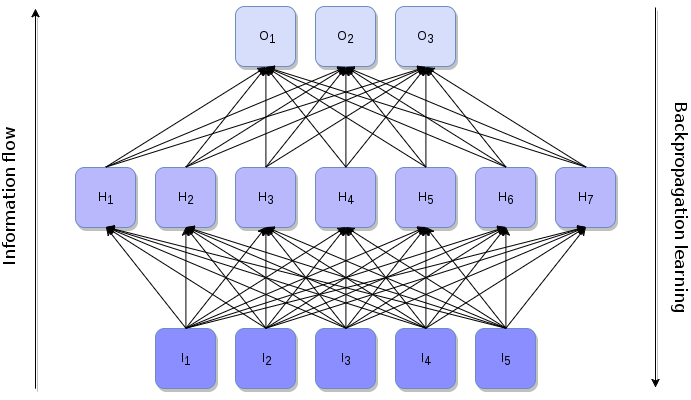
\includegraphics[width=0.9\textwidth]{gfx/NeuralNetwork.png}
        \caption{A neural network with one hidden layer.}

    \end{figure}

    We can see that the hidden layer has its neurons labeled $H_i$. The input layer is represented by the $I_i$ units and the output layer corresponds to the different $O_i$. 

    This image introduces another new concept: \textit{backpropagation}. Whereas the information is transformed by means of the weights and transmitted forward, the adjustment of those weights also needs of a propagation in the opposite direction. To sum it up, backpropagation has two main steps:

    \begin{enumerate}

    	\item
    	Propagation. Generate predictions for the training examples, then calculate the error at the output layer; a common error measure is the squared difference between the actual value and the expected value. Afterwards, recursively propagate the error calculations to the successive hidden layers taking into acount the already computed error values, until the input layer is reached.

    	\item
    	Weight update. Multiply the value of the activation function of each neuron and its error obtained in the first step. This is called the \textit{gradient} in \textit{Gradient Descent}. Finally, subtract a fraction of this gradient from the weight; that fraction (\textit{learning rate}) has a significant effect on the process, for a value too high can cause the algorithm to jump over a local minimum without reaching it, and a value too low can overextend the training time.

    \end{enumerate}

    The above procedure is repeated until the model's performance is adequate. If we wish to speed it up with a reasonable tradeoff in quality, we can use not the whole training set for each iteration but smaller subsets called \textit{batches} (\textit{Stochastic Gradient Descent}). This allows us to maintain enough generalization while at the same time reducing the cost of gradient computation \cite{lecun-dl}.

    A problem related to backpropagation is the \textit{vanishing gradient}, which only occurs in the training stage of neural networks. Because of the chain rule used to propagate the error through the layers, if the activation function has a near-zero derivative at some points, the gradient will approach that value too. In worst-case scenarios, it results in a practical standstill of the training.

    Multiple solutions have been proposed in the past few years, and research on the topic is still ongoing. A few popular activation functions as of now include:

    \begin{itemize}

    	\item
    	\textit{Hyperbolic tangent}: the classic, due to it being bounded, which increases the efficiency of the training. However, its shape at both ends produces the vanishingly small gradients.

    	\item
    	\textit{\ac{ReLU}}: defined by $f(x) = 0$ if $x \leq 0$ and $f(x) = x$ if $x > 0$. It avoids small gradients for high input values and makes networks sparser with its negative part (accounting again for more efficiency). The downside is the \textit{dying} \acs{ReLU}, in which some neurons become perpetually inactive.

    	\item
    	\textit{Leaky \acs{ReLU}}: one of the variants of \acs{ReLU} which tries to avoid inactive neurons by setting $f(x)$ for negative $x$ to $0.01x$ instead of $0$. Its generalization is the \textit{Parameterized ReLU} \cite{delv-deep-relu,deep-res-relu}.

    	\item
    	\textit{\ac{ELU}} \cite{elu}: another recent alternative that replaces the horizontal section of the \acs{ReLU} with an exponential function.

    \end{itemize}

    These functions can be observed in the following figure:

    \vspace{0.2cm}

    \begin{figure}[bth]

        \myfloatalign
        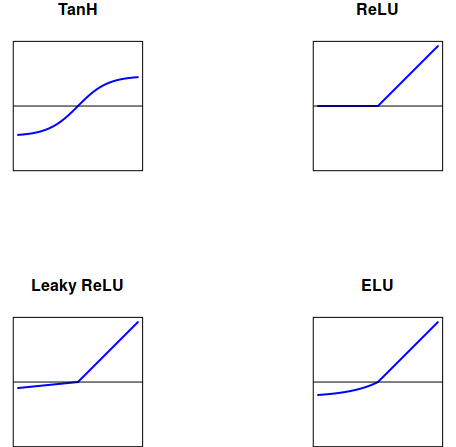
\includegraphics[width=0.7\textwidth]{gfx/ActivationFunctions.png}
        \caption{Four of the most popular activation functions.}

    \end{figure}

    In general, as the complexity of a model grows, so does the difficulty of its training. Neural networks are, in theory, capable of approximating every possible function, and this comes at a price: some of the following common issues in machine learning \cite{nn-atc} have increased consequences.

    \begin{itemize}

    	\item
    	Limited data: without delving too much into the underlying theory, the more powerful a model is, the more training samples are needed in a substantial proportion. Coupled with it, the smaller the training set, the smaller the chance it will represent the whole population.

    	\item
    	Imbalanced data: when there are far more examples of one or more classes than of the rest, we speak of imbalance. Apart from not representing the population, this phenomenon can even bias a classifier in a way that it only outputs one class, as it seems the best way to minimize the error.

    	\item
    	Incomplete data: this is the case when the available samples have missing values. In this situation there are two options: either we discard incomplete fields from across all samples or we try to infer them.

    	\item
    	High dimensionality: linking with the first bullet point, powerful models can suffer of \textit{overfitting} with limited and/or high-dimensional samples. The latter can cause the model to just learn the available data ``by heart'' and fail to generalize to new examples. Even leaving extreme cases aside, the number of features has a direct impact on the time required for training.

    \end{itemize}

    It is clear that we must minimize the hurdles posed by the data, and also make sure we pick the right parameters. For this second task, we have \acf{EA}.

\section{Evolutionary algorithms}\label{sec:genetic_algorithms}

	Evolutionary algorithms are iterative procedures that take a population of feasible solutions to a problem and try to progressively find the best possible answer by mimicking nature in its selection process. 

	Being general-purpose metaheuristics, they find use in fields as disparate as computer science, medicine, economics or cryptography, among many others. In the business at hand, they will serve as neural network optimizers, in addition to feature selectors in a preliminar step.

\newpage

	The kind of \acs{EA}s we will be using are known as \textit{genetic algorithms}. Now, if we analyze them, we find they have several main pieces:

	\begin{itemize}

		\item
		Individual: a potential solution to a problem, represented in an adequate manner.

		\item
		Population: a set of individuals for a given iteration (\textit{generation}).

		\item
		Fitness: every genetic algorithm has one or more fitness functions which evaluate the quality of an individual. It can be the most expensive operation, depending on the situation.

		\item
		Selection process: the creation of new individuals (\textit{offspring}) needs a set of parents. The selection process chooses them based on some criteria, usually involving the fitness.

		\item
		Crossover operator: once we have a list of potential parents, this operator defines how to create \textit{offspring} that resemble them in some way.

		\item
		Mutation operator: in order to maintain diversity, random mutations are introduced with a certain probability.

		\item
		Replacement: how the old population and the offspring set will be used to create a new population.

	\end{itemize}

	Strong emphasis is placed on a solid balance between finding novel solutions and improving the best ones yet, also known as the \textit{exploration-exploitation tradeoff}. Hence, all the pieces as a whole must attain a delicate synergy. With that in mind, let us go into a bit more detail in the next sections.

	\subsection{Individuals}

		The individuals of a genetic algorithm may be represented in a variety of ways. It is crucial to find the best suited for our needs, as it will not only impact time and space efficiency but also the overall performance of the optimization, enabling some genetic operators and discarding others.

		For example, in feature selection we could code our solutions as a binary vector in which the ones represent active features and the zeros inactive features. Alternatively, we could just keep a list of the indices of active features; this would use less memory but also make some very simple operators in binary codification way more convoluted to implement.

		Common representations include binary, order-based and real-valued. Having already exemplified the first, order-based is natural in \textit{Travelling Salesman Problem}-like cases and real-valued can be found in numerical function optimization.

	\subsection{Population}

		Population size must have an equilibrium between enough individuals to explore the solution space and not too many of them, which would lead to excessive running times.

		Another relevant discussion is how to initialize the first set of individuals. For the sake of a good exploration, it should include a decent portion of the search space, often taking advantage of randomness.

	\subsection{Fitness}

		Fitness measures, both in type and in number, depend on what aspect of a problem we want to tackle. 

		If we hope to find a global maximum or minimum in a complex function, the fitness will just compute the value at a given point. If we want to choose from a set of features, the evaluation will need to assess how good a subset is by training and testing a machine-learning model; similarly, if we wanted to further optimize that model, we would need to try many variations of its parameters.

		However, suppose we can't decide on what we prefer to improve: for instance, we want a solution to be as accurate as possible, but we want it to be simple, too. This is when \textit{multiobjective optimization} comes in: instead of returning the best candidate, we accept a compromise between the two criteria and return a list of candidates that are not better or worse than the others. They just score well in both measures but in different proportions.

	\subsection{Selection}

		Parent selection process is one of the keys for the success or failure of the algorithm. Since it is a problem-independent part of the algorithm, in contrast with the more specific crossover and mutation operators, we can reduce our choices to a handful of classic techniques \cite{selection-ga}:

		\begin{itemize}

			\item
			Proportional: the probability of picking an individual is driven by its relative fitness with respect to the overall sum.

			\item
			Tournament: $n$ random individuals are set side by side and compared by fitness score, after which the best is taken. Repeat until the parent quota is met.

			\item
			Ranking (any kind): with the population sorted by fitness, it assigns order-based probabilities following some function. The catch here is that the probabilities are not directly related to the measured quality of the solutions, which allows for more control over convergence-exploration.

			\item
			Randomized: little to no influence of fitness in the decision.

		\end{itemize}

	\subsection{Crossover}

		There exist a plethora of options for this highly representation-dependent operator. As it is unfeasible to list them all, even just the most relevant ones, we will limit this section to the kinds we will use. The only prerequesite is that they offer a degree of continuity from parent to offspring.

		\subsubsection{In binary representation}

			Like we mentioned earlier, a binary representation consists of a series of zeros and ones. While not the most memory-efficient alternative, it results in fairly straightforward yet powerful operators:

			\begin{itemize}

				\item
				Single-point: choose a random position between the first and the last. To each of its sides we only add the elements of a single parent.

				\vspace{0.2cm}

			    \begin{figure}[bth]

			        \myfloatalign
			        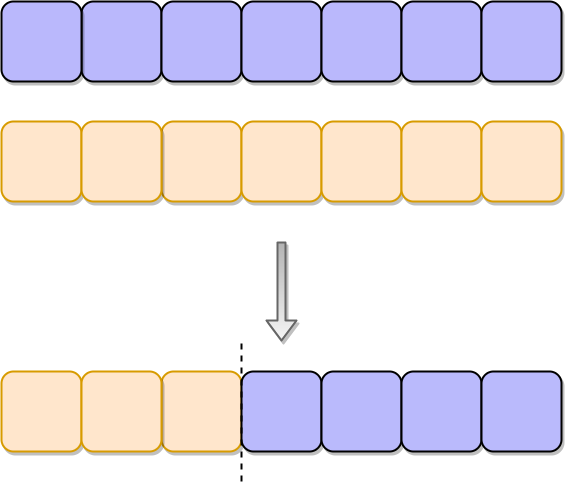
\includegraphics[width=0.5\textwidth]{gfx/SinglePointCrossover.png}
			        \caption{Single-point crossover example.}

			    \end{figure}

			    \item
			    Double-point: this time, generate two random positions. Use them to alternate the two parents' elements. Note that this idea can be extended to $n$-point crossovers.

			    \vspace{0.2cm}

			    \begin{figure}[bth]

			        \myfloatalign
			        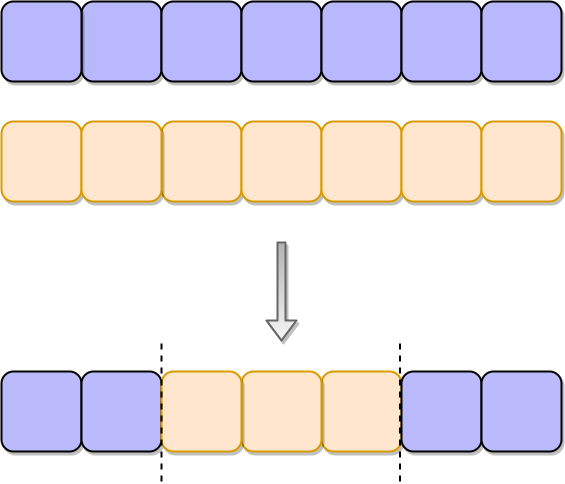
\includegraphics[width=0.5\textwidth]{gfx/DoublePointCrossover.png}
			        \caption{Double-point crossover example.}

			    \end{figure}

			    \item
			    Uniform (UX): choose a uniform real number between 0 and 1 and use it to decide which of the two parents the $ith$ bit will come from. From a practical standpoint, this means that bits shared by both of them will always be passed on to the next generation.

			    \vspace{0.2cm}

			    \begin{figure}[bth]

			        \myfloatalign
			        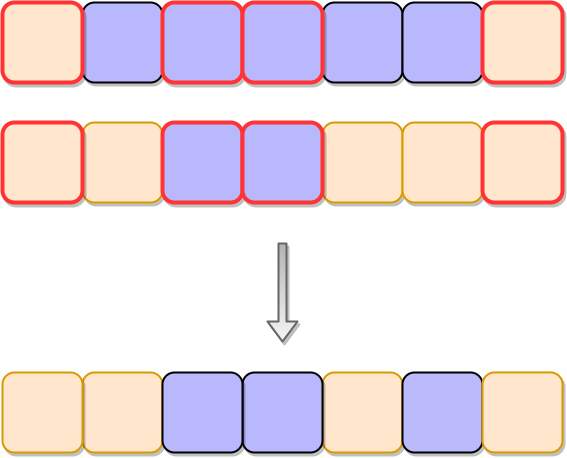
\includegraphics[width=0.5\textwidth]{gfx/UniformCrossover.png}
			        \caption[Uniform crossover example.]{Uniform crossover example. Note that the highlighted elements are present in both individuals.}

			    \end{figure}

			\end{itemize}

		\subsubsection{In neural networks}

			If binary representations and crossovers are among the most widely studied, it is not quite the case with neural networks in genetic algorithms (probably because the revival of the field happened not many years ago).

			Some parameters (\textit{hyperparameters}, because their values are fixed before the training phase) to tune are the number of hidden layers, or neurons per layer, or the learning rate.

			For the first two, one could do something along the lines of the binary crossovers we just explained: take some layer sizes from one parent and the rest from the other, have the child get as many hidden layers as the average of its parents, etc. Perhaps we want to keep the numbers inside tolerance intervals, so we should check after each operation too.

			To pass learning rates on, maybe a simple average would do. Given that we don't have prior knowledge about the function we are trying to optimize---only that it has a global optimum somewhere---, it would be a reasonable strategy: if the optimum is between two values, an average would keep us in range; if not, we would not have known anyway.

\newpage

	\subsection{Mutation}

		Evolution needs some diversity, and what we have not done with selection and crossover, we must do with mutations in the offspring.
		Again, the mutation operator can take many forms, so we will restrict ourselves to what is applicable.

		\subsubsection{In binary representation}

			The easiest way to mutate a vector of binary elements is to randomly flip one or more of them i.e. write 1 where there was 0 and viceversa. Both the amount of flips and the probability of a mutation rule how much diversity is introduced.

		\subsubsection{In neural networks}

			When dealing with quantities, such as the number of layers or of neurons per layer, the simplest thing to do is to add or subtract. A more frequent mutation could be to just alter the number of neurons in one (or more than one) layer either by a fixed amount or by using a probability distribution (gaussian noise, for instance). A much rarer mutation---for its impact in the structure of the network---could involve a slight change in the number of layers.


	\subsection{Replacement}

		The act of combining the old population and the freshly-created offspring into a new population for the next generations has a great significance in the final outcome of the algorithm. Let us start reviewing the two categories of genetic algorithms according to the magnitude of the replacement:

		\begin{itemize}

			\item
			Steady-state: only a few parents---typically two---are selected for reproduction in each generation, and the offspring they yield replace the same amount of individuals in the original population.

			\item
			Generational: the whole previous population is displaced by a newly created group.

		\end{itemize}

		Since these categories are not strict, we could have a genetic algorithm that ranks halfway between the two: not all the previous individuals have to be replaced. We usually make this decision with the help of additional criteria: imagine that we lump together all the individuals and sort them by fitness; all offspring could be better than the best old individual, and thus the entire population would be replaced, but it might very well not be the case, and end up with a mix of old and new.

		The way in which we choose to do the replacement causes, along with the selection procedure, a certain degree of \textit{selective pressure} \cite{selection-ga}. Selective pressure characterizes the extent to which better individuals are prioritized in the evolution stages of the algorithm.

		Finally, here is a graphic overview of how a genetic algorithm works:

		\vspace{0.2cm}

	    \begin{figure}[bth]

	        \myfloatalign
	        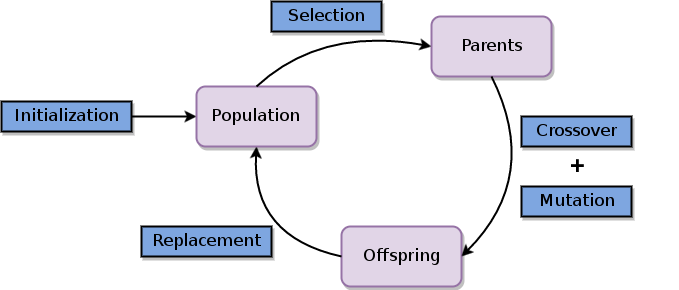
\includegraphics[width=0.9\textwidth]{gfx/GeneticAlgorithm.png}
	        \caption[Structure of a genetic algorithm.]{General overview of a cycle in a genetic algorithm. Blue boxes represent operations. Violet boxes represent sets of individuals.}

	    \end{figure}

	    It is important to note that this basic scheme is complemented by the stopping conditions, which range from finding the optimum (when we have the number but need the associated solution) to an artificial limit by iteration count or a streak of non-productive generations.

\section{Multiobjective optimization}

	As was briefly discussed in a previous section, it is possible to have several criteria to guide our search of good solutions for our problem.

	We can define multiobjective optimization in a more formal way:

	\begin{equation}
		\min_{x \in X}(f_1(x),f_2(x),...,f_n(x))
	\end{equation}

	Where $X$ represents the space of possible solutions, and $n > 1$ is the number of objective functions. An alternative notation would be taking $F(x)$ as a vectorial function containing all $f_n(x)$.

	When looking for suitable solutions, we pay special attention to \textit{Pareto-optimal} solutions, which are \textit{non-dominated}. Domination of $x_1$ over $x_2$, with $x_1,x_2 \in X$, can be defined by the following two conditions:

	\begin{enumerate}

		\item
		$f_i(x_1) \leq f_i(x_2), \forall i : 1\leq i \leq n$

		\item
		$f_i(x_1) < f_i(x_2),$ for one or more $i \in \{1,2,...,n\}$

	\end{enumerate}

\newpage

	The \textit{Pareto front} is the set of solutions which meet both conditions for the rest of solutions but fail to meet the first one when compared among themselves. An example of a Pareto front is shown in the next figure:

	\vspace{0.2cm}

	\begin{figure}[bth]

        \myfloatalign
        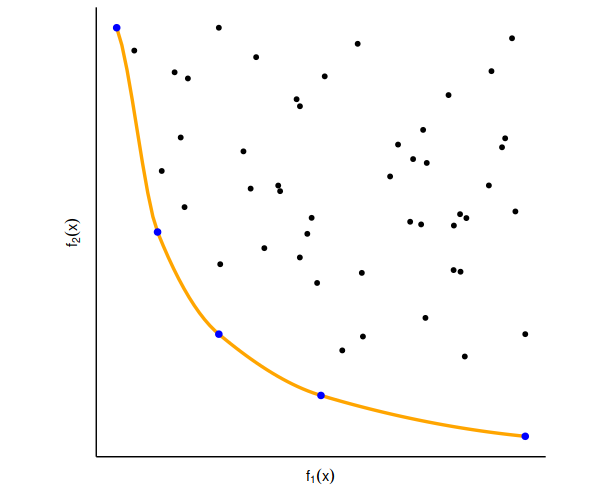
\includegraphics[width=0.75\textwidth]{gfx/ParetoFront.png}
        \caption[An example of Pareto front.]{A two-dimensional Pareto front with its points highlighted in blue and an approximate curve outlined in orange.}

    \end{figure}

    A multiobjective optimization algorithm typically returns the Pareto front in its entirety, and it is our duty to make an informed decision about which element(s) we deem more appropriate.

\section{Feature selection}

	When we face a complex classification or regression job, we often have a lot of unorganized information. In these cases, one of the keys for success is to weed out whatever data that does not contribute anything useful. An excess of data does not just increase the computational cost of training our models, it can also hamper its performance---and in no small proportion, to make things worse.

	It is therefore clear that we need some kind of method for choosing the right information to keep. However, achieving this is no easy feat, as it falls into the category of \textit{NP-hard} problems \cite{amaldi1998approximability}. For this reason, a number of approximate alternatives have been proposed. They can be of one of three classes \cite{guyon2003introduction}.

	\textit{Wrappers} use the performance of a model to score different feature subsets. \textit{Filters} select features as a preprocessing step, independent from any models we later use. \textit{Embedded} methods incorporate the selection in their training processes. Wrappers tend to yield the best outcomes because of their more extensive search, and are a good option if given enough computational resources; with these conditions met, we will be using genetic algorithms, a popular example.

	As we want to have more than one measure of classification quality, we will use a multiobjective genetic algorithm. Picking up on what we said in the last section, Pareto-based approaches are quite common. Among these, the state of the art is mainly comprised of some of the most famous algorithms: \ac{NSGA-II} \cite{deb2002fast}, \ac{SPEA2} \cite{zitzler2001spea2} and \ac{PAES} \cite{knowles1999pareto}. 

	The first one is the most widely used by a large margin, and we will use it too for two main reasons: its higher general performance against the other alternatives, along with its better population diversity (refer to the original paper for more details), is a decisive factor; in addition, since it works with a single population instead of keeping a concurrent one for the best individuals, it is easier to implement and conceptually more intuitive.

	One important downside of multiobjective genetic algorithms is, though, that they do not perform so well with many objectives. But, since we will use a maximum of two or three, it should not become a problem for us.
	\chapter{Motivation and objectives}\label{ch:objectives} 
%************************************************

\section{Motivation}

	In recent years, the field of machine learning has seen substantial advances. Due to the emergence of a wide array of novel techniques and the significant increase in computational power, state-of-the-art models outperform older methods in many applications. Deep Neural Networks are the most successful example, achieving results comparable to those of humans in tasks such as image recognition or game playing.

	Because of this, a certain degree of knowledge or familiarity with machine learning is a valuable asset for any Computer Science or Computer Engineering graduate. Thus, this work aims to serve as an opportunity to acquire more insight into the capabilities of neural networks in conjunction with related optimization methods. Additionally, since we will be using real data instead of typical testing datasets, it will provide some experience about tangible problems and their complexity.

	My personal motivation is not too far from the above. As a sci-fi reader, the idea of machines solving tasks better than humans is always present. True machine intelligence may not come soon, if it ever does, since there is a long road ahead; however, experience demonstrates that we are too early to either dismiss or take for granted, and so the only way to know is to try, step by step. Although not as fancy as what can be found in \textit{Hugo} and \textit{Nebula} award winners, machine learning is already a reality in terms of usefulness, and that is what I am interested in.
	\part{Methodology}\label{pt:methodology}
	\chapter{The dataset}\label{ch:dataset}
%************************************************

\section{Description}

	As stated in Chapter \ref{ch:context}, we will be working with \acs{EEG} readings. The patterns have been built using a kind of \ac{MRA} \cite{daubechies1992ten} called the \ac{DWT}, applied in \cite{asensio2013multiresolution} to characterize \acs{EEG}s from \ac{MI} tasks. On this occasion, our aim is to use them to distinguish between an imagined movement of the left hand, the right hand or the feet.

	The feature extraction procedure yields a variable but always huge number of coefficients. This number is determined by:

	\begin{itemize}

		\item
		$S$: number of segments.

		\item
		$E$: number of electrodes.

		\item
		$L$: number of levels.

	\end{itemize}

	If we input them in the formula $2 \times S \times E \times L$, we obtain how many sets of coefficients describe the pattern. In turn, each set can contain from 4 to 128 coefficients. For the experiment at hand, $S = 20$, $E = 15$ and $L = 6$, making a total of 3600 sets and the overall limit being 151200 features.

	Again, \cite{asensio2013multiresolution} proposed a way of reducing this amount by computing the variance of each set, leaving us with 3600 features altogether.

	Whereas this is a massive reduction in dimensionality, the scarcity of sample patterns (about 360 in total) still poses a challenge for the task of classification at hand.

\section{The curse of dimensionality} 

	When dealing with high-dimensional spaces (those with hundreds or thousands of dimensions), we face issues that are often not present in simpler ones. As the volume of the space grows, the samples become sparser and thus they fail to represent the whole set of possibilities in a statistically significant way.

	Applied to machine learning, the number of features plays a pivotal role: a low count may not provide enough information, and a high count may prevent a good generalization by introducing superfluous or noisy details. Thus, the key lies somewhere in the middle: we have to find a delicate balance so that our models do not \textit{underfit} nor \textit{overfit}. 

\newpage

	The latter is our main concern when trying to bring down the feature count, so we will restrict ourselves to a subset smaller than the training one. Since we are going to split the (approximately) 360 samples evenly for training and testing, this means that we should consider at most 180 features--ideally, only a fraction of that.

	As a final note, it is important to mention that we have several instances of this dataset structure that correspond to different test subjects (namely, 104, 107 and 110). These subjects were the best performers in the recordings, because one of the downsides of \acs{EEG} and \acs{MI} is that the person has to learn how to use the device. The other subjects were not so good at the task, and so they will not be considered here.
	\chapter{Feature selection}\label{ch:featureselection}
%************************************************

Like we mentioned before, the chosen approach for the feature selection step is a genetic algorithm. With a few modifications specific to our problem, the basic structure will be that of \acs{NSGA-II}.

We previously hinted in chapter \ref{ch:background} at a binary representation when dealing with this kind of task. It not only facilitates the overall implementation, but---as we already said---it also brings with it some easy yet effective operators.

\section{Feature selection procedure}

	The main body of the algorithm corresponds to a typical \acs{NSGA-II} layout. We will see its general form before going over the different parts:

	\vspace{0.2cm}

	\begin{algorithm}[H]

		\Proc{NSGA-II($population\_size$, $generations$, $data$, $max\_features$)}{

			population $\longleftarrow$ Initialize(population\_size,max\_features)\;
			evaluation $\longleftarrow$ Evaluate(population,data)\;
			sorting $\longleftarrow$ NonDominatedSort(population,evaluation)\;
			
			\For{$gen = 0$ \KwTo $total\_generations$}{
			}
		}

		\caption{NSGA-II}

	\end{algorithm}



	\chapter{Neural network optimization}\label{ch:optimization}
%************************************************ 

The definition of hyperparameter is often fuzzy. In this work, we view hyperparameters as those parameters which are fixed before training a model, because there are no direct rules to infer them from the available data. In fact, we probably would not need them at all if we had enough data, since the samples would tell us everything that is to be known about a given problem. As we will almost never find ourselves in such a favorable situation, there exists a real need to find the right combination of hyperparameters for the circumstances at hand.

One could understand feature selection as a form of hyperparameter optimization, since it is in a way fixing a part of the model---the entry point of the data. It is undoubtedly a key tool when dealing with an absurd quantity of decision variables and, whether it is hyperparameter optimization or not, it already has a section in its own right. From here on, we will focus on tuning aspects specific to neural networks, such as the learning rate, the number of epochs in training or the dropout rate \cite{srivastava2014dropout}.
	\part{Experiments and conclusions}\label{pt:results}
	\chapter{Experimental results}\label{ch:experiments}
%************************************************ 

In this chapter, we start by detailing in section \ref{sec:technologies} the choice of technologies in order to obtain experimental results. After that, these results will be discussed in order of application in sections \ref{sec:res_fs} (feature selection), \ref{sec:res_so} (structure optimization) and \ref{sec:res_lo} (learning optimization). By the end, we will have empirical evidence to point us in promising directions, which we will subsequently address when we talk about conclusions and future work.

\section{Software and hardware}\label{sec:technologies}

	\subsection{Software}

		The first decision to make is which programming language to use. \texttt{Python} is the choice for the following reasons:

		\begin{itemize}

			\item
			Previous experience with the language in web and machine learning applications.

			\item
			Popularity of the language, which is a good indicator of community support. According to the \textit{StackOverflow} 2018 Survey \footnote{\href{https://insights.stackoverflow.com/survey/2018/\#technology-programming-scripting-and-markup-languages}{\textit{StackOverflow} 2018 Survey: Most popular technologies}}, it is one of the most popular languages, and more so if we compare it with those commonly associated with machine learning in the last few years.

			\item
			Popularity of its machine learning and deep learning frameworks. Well-established frameworks include \texttt{Scikit-learn} \footnote{\href{https://github.com/scikit-learn/scikit-learn}{\texttt{Scikit-learn} GitHub repository}}, \\ \texttt{Caffe} \footnote{\href{https://github.com/BVLC/caffe}{\texttt{Caffe} GitHub repository}}, \texttt{TensorFlow} \footnote{\href{https://github.com/tensorflow/tensorflow}{\texttt{TensorFlow} GitHub repository}} and \texttt{Theano} \footnote{\href{https://github.com/Theano/Theano}{\texttt{Theano} GitHub repository}}. The last two of them also function as backends for the high-level neural networks API \texttt{Keras} \footnote{\href{https://github.com/keras-team/keras}{\texttt{Keras} GitHub repository}}. If we look at the number of stars in their \textit{GitHub} repositories, we can see that they are widely acknowledged by the community.

		\end{itemize}

\newpage

		The next step is choosing the tools to support our work. Since one of the goals of this project was to learn about optimization techniques, the genetic algorithm has been implemented from scratch, although there are alternatives like \texttt{DEAP} \footnote{\href{https://github.com/DEAP/deap}{\texttt{DEAP} GitHub repository}} if one wishes to avoid the additional development effort.

		Data operations become faster and easier with \texttt{Numpy} \footnote{\href{https://github.com/numpy/numpy}{\texttt{Numpy} GitHub repository}}. This will allow us to manage populations in genetic algorithms, as well as perform basic operations in a vectorized way whenever we need them. It is also fully compatible with the other libraries.

		Building machine learning models from scratch too is understandably out of the question. For this reason, we will rely on \texttt{Scikit-learn} for general machine learning algorithms and metrics, and on \texttt{Keras}---with its default \texttt{TensorFlow} backend---for neural networks.

		Lastly, many charts will be generated using \texttt{R} \footnote{\href{https://www.r-project.org/}{\texttt{R} Project website}}, which provides simple and powerful functionality for this task.

	\subsection{Hardware}

		We can make a distinction in this regard between the main development system, used for testing and debugging, and the dedicated servers for full-scale experimentation:

		\begin{itemize}

			\item
			Development system:

			\begin{itemize}

				\item
				Intel® Core™ i5-3470 CPU @ 3.20GHz, 8GB DDR3.
				\item
				NVIDIA GeForce® GTX 960, 2GB GDDR5.

			\end{itemize}

			\item
			First dedicated server:

			\begin{itemize}

				\item
				Intel® Xeon® E5-2620 v2 @ 2.10GHz, 32GB DDR3.
				\item
				NVIDIA Tesla® K20c, 5GB GDDR5.

			\end{itemize}

			\item
			Second dedicated server:

			\begin{itemize}

				\item
				Intel® Xeon® E5-2620 v4 @ 2.10GHz, 32GB DDR4.
				\item
				NVIDIA Tesla® K40m, 12GB GDDR5.

			\end{itemize}

			\item
			Third dedicated server:

			\begin{itemize}

				\item
				Two Intel® Xeon® E5-2620 v4 @ 2.10GHz, 32GB DDR4.
				\item
				NVIDIA Tesla® K40m, 12GB GDDR5.

			\end{itemize}

		\end{itemize}

\newpage

\section{Feature selection}\label{sec:res_fs}

	Determining the right configuration for the genetic algorithm---or rather, even one that is good enough---is no trivial task. Early experimentation seemed to point to a high crossover probability, but especially to a high mutation probability (ultimately set to 1). We will elaborate on that soon.

	Let us start by comparing three different crossover operators: \textit{Uniform}, \textit{Single-point} and \textit{Two-point}. We will work with a population of 300 individuals and 150 generations. We will set a 0.9 crossover probability after which a mutation will always ensue. A maximum of 50 active features will be allowed in each individual. The fitness criteria will take into account the Kappa value (for test accuracy) and a 5-fold cross-validation (for generalization assessment) measured for Logistic Regression.

	We will do an initial test run on each subject (104, 107 and 110). 

	Figure \ref{gfx:fs_crossover_kappa} displays the evolution of the mean Kappa error for all crossover operators in all three subjects.

    \begin{figure}[h]

        \begin{center}

        	\setlength{\fboxrule}{0pt}
            \fbox{
				\begin{varwidth}{\textwidth}
					\centering
					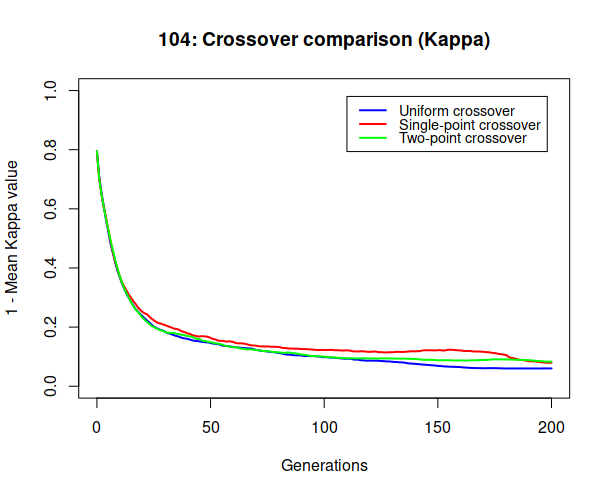
\includegraphics[width=0.45\textwidth]{gfx/FS_Crossover_Kappa_104.png}
				\end{varwidth}
			}
			\fbox{
				\begin{varwidth}{\textwidth}
					\centering
					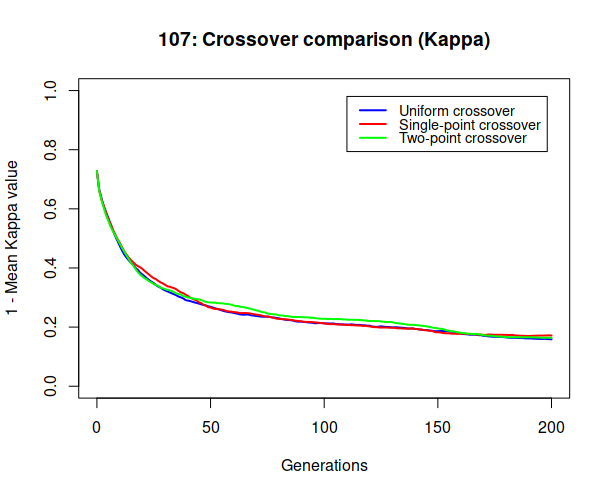
\includegraphics[width=0.45\textwidth]{gfx/FS_Crossover_Kappa_107.png}
				\end{varwidth}
			}
            \fbox{
				\begin{varwidth}{\textwidth}
					\centering
					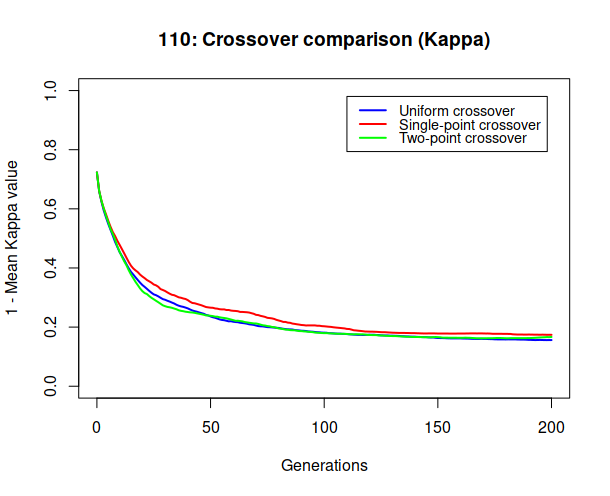
\includegraphics[width=0.45\textwidth]{gfx/FS_Crossover_Kappa_110.png}
				\end{varwidth}
			}

		\end{center}
		\caption[Kappa loss comparison for different crossovers]{Comparison of Kappa loss evolution over time with different crossover operators.}\label{gfx:fs_crossover_kappa}

	\end{figure}

	We can identify appreciable differences between the three curves: the blue one (uniform crossover) shows consistently better results than the other two, and the red one (single-point crossover) appears to be the worst.

\newpage

	Let us move on now to the same type of chart but with the cross-validation error (Figure \ref{gfx:fs_crossover_cv}). Again, the uniform crossover operator achieves the top performance across all individuals and the single-point crossover operator often lags behind.

	\begin{figure}[h]

        \begin{center}

        	\setlength{\fboxrule}{0pt}
            \fbox{
				\begin{varwidth}{\textwidth}
					\centering
					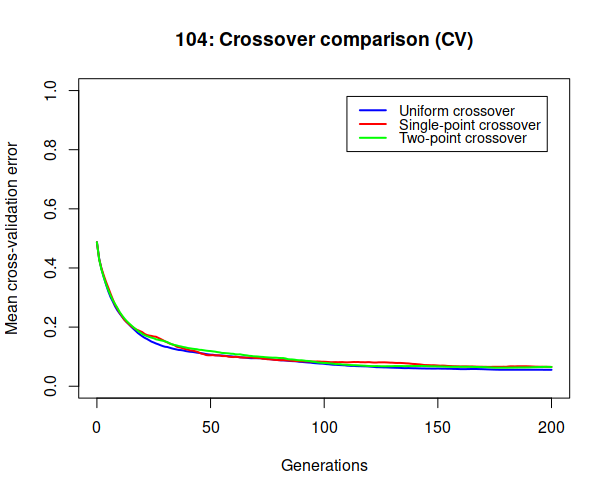
\includegraphics[width=0.45\textwidth]{gfx/FS_Crossover_CV_104.png}
				\end{varwidth}
			}
			\fbox{
				\begin{varwidth}{\textwidth}
					\centering
					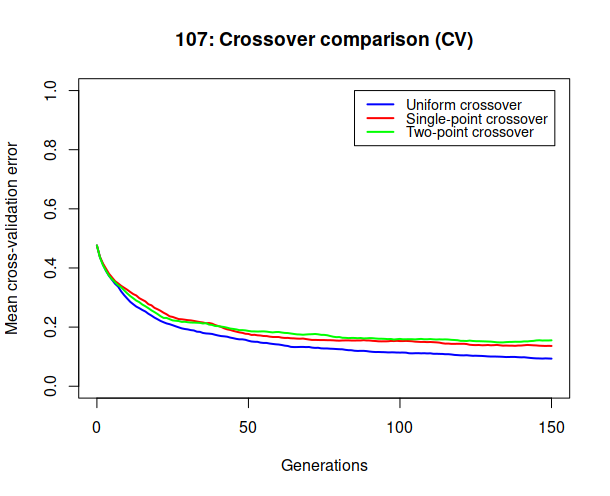
\includegraphics[width=0.45\textwidth]{gfx/FS_Crossover_CV_107.png}
				\end{varwidth}
			}
            \fbox{
				\begin{varwidth}{\textwidth}
					\centering
					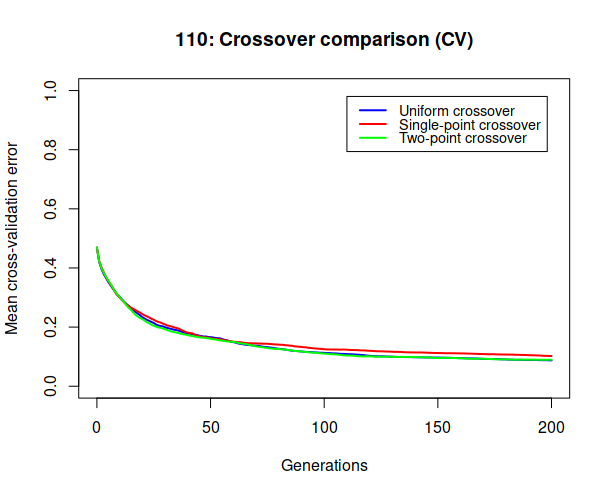
\includegraphics[width=0.45\textwidth]{gfx/FS_Crossover_CV_110.png}
				\end{varwidth}
			}

		\end{center}
		\caption[CV loss comparison for different crossovers]{Comparison of cross-validation loss evolution over time with different crossover operators.}\label{gfx:fs_crossover_cv}

	\end{figure}

	We seem to be spotting a trend that depends on the crossover operator. However, is it wise to extrapolate from only one test run? The answer is no: the running times allow us to repeat the experiment several times and find out whether their differences are statistically significant.

	As a compromise between quantity of samples and time expended, we will analyze 15 samples per crossover operator using their Kappa error values. Table \ref{table:crossover_kappa} shows the resulting values for all possible combinations:

	\vspace{0.3cm}

	\begin{table}[h]

        \centering
        \setlength\arrayrulewidth{0.8pt}

        \begin{tabular}{| >{\centering\arraybackslash}m{0.5in} | >{\centering\arraybackslash}m{1.1in} | >{\centering\arraybackslash}m{1.1in} | >{\centering\arraybackslash}m{1.1in} |}

            \hline
            \rowcolor{RoyalBlue}
            \textbf{Subject} & \textbf{Uniform} & \textbf{Single-point} & \textbf{Two-point} \\
            \hline
            \textbf{104} & $0.06534 \pm 0.0074$ & $0.08619 \pm 0.0102$ & $0.07941 \pm 0.0119$ \\
            \hline
            \textbf{107} & $0.15202 \pm 0.0132$ & $0.18004 \pm 0.0137$ & $0.17725 \pm 0.0150$ \\
            \hline
            \textbf{110} & $0.14829 \pm 0.0138$ & $0.17131 \pm 0.0158$ & $0.16569 \pm 0.0187$ \\
            \hline

        \end{tabular}

        \caption{Comparison of average Kappa error values for the three subjects and the three crossover operators.}\label{table:crossover_kappa}

    \end{table}

    The average performance of each operator seems to be what we expected. Additionally, the uniform crossover appears to produce slightly more stable results, judging from the standard deviation. Next, and not making assumptions about normality, we will perform a \textit{Kruskal-Wallis} test to see if their differences are worth considering. The \textit{p-values} are displayed in Tables \ref{table:crossover_kruskal_104}, \ref{table:crossover_kruskal_107} and \ref{table:crossover_kruskal_110}, with values below $0.05$ representing meaningful differences ($95\%$ confidence interval).

	\begin{table}[h]

        \centering
        \setlength\arrayrulewidth{0.8pt}

        \begin{tabular}{| >{\centering\arraybackslash}m{0.9in} | >{\centering\arraybackslash}m{0.9in} | >{\centering\arraybackslash}m{0.9in} |}

            \hline
            \rowcolor{RoyalBlue}
            \textbf{104} & \textbf{Single-point} & \textbf{Two-point} \\
            \hline
            \cellcolor{RoyalBlue}\textbf{Uniform} & $p = 0.000027$ & $p = 0.000835$ \\
            \hline
            \cellcolor{RoyalBlue}\textbf{Single-point} & \cellcolor{lightgray} & \textcolor{red}{$p = 0.056282$} \\
            \hline

        \end{tabular}

        \caption{Comparison of p-values for the crossover operators (subject 104).}\label{table:crossover_kruskal_104}

    \end{table}

    \begin{table}[h]

        \centering
        \setlength\arrayrulewidth{0.8pt}

        \begin{tabular}{| >{\centering\arraybackslash}m{0.9in} | >{\centering\arraybackslash}m{0.9in} | >{\centering\arraybackslash}m{0.9in} |}

            \hline
            \rowcolor{RoyalBlue}
            \textbf{107} & \textbf{Single-point} & \textbf{Two-point} \\
            \hline
            \cellcolor{RoyalBlue}\textbf{Uniform} & $p = 0.000023$ & $p = 0.000104$ \\
            \hline
            \cellcolor{RoyalBlue}\textbf{Single-point} & \cellcolor{lightgray} & \textcolor{red}{$p = 0.678133$} \\
            \hline

        \end{tabular}

        \caption{Comparison of p-values for the crossover operators (subject 107).}\label{table:crossover_kruskal_107}

    \end{table}

    \begin{table}[h]

        \centering
        \setlength\arrayrulewidth{0.8pt}

        \begin{tabular}{| >{\centering\arraybackslash}m{0.9in} | >{\centering\arraybackslash}m{0.9in} | >{\centering\arraybackslash}m{0.9in} |}

            \hline
            \rowcolor{RoyalBlue}
            \textbf{110} & \textbf{Single-point} & \textbf{Two-point} \\
            \hline
            \cellcolor{RoyalBlue}\textbf{Uniform} & $p = 0.000454$ & $p = 0.006561$ \\
            \hline
            \cellcolor{RoyalBlue}\textbf{Single-point} & \cellcolor{lightgray} & \textcolor{red}{$p = 0.299489$} \\
            \hline

        \end{tabular}

        \caption{Comparison of p-values for the crossover operators (subject 110).}\label{table:crossover_kruskal_110}

    \end{table}

    As we can see, the single-point and two-point crossovers show no statistically significant differences in their recorded results.

    The computational impact of either operator is negligible against the much more intensive fitness evaluations, so there is no reason not to consider the uniform crossover as our pick from now on. The last thing to do before moving on is attempt to explain why this happens. 

    On one hand, $n$-point crossovers merge large blocks from both parents; this leads to a not-so-optimal information transfer when trying to pick a handful of features from a pool of 3600.

    On the other hand, the uniform crossover is often said to be very disruptive, due to randomly choosing elements for which the parents do not agree. However, when only a small portion $k$ of features is active at a time, the disruption is at most $2k$ elements (the rest are inactive features); on top of that, features in which both parents agree are always kept. This makes the uniform crossover excel at \textit{exploitation} while also helping in \textit{exploration}. Together with frequent mutations, this is probably the key of the performance gain of the algorithm.

    Another aspect to look into is the effect of population sizes and number of generations. Bigger populations should introduce greater exploration possibilities, while more generations should allow the genetic algorithm to converge to even better solutions. Nevertheless, an increase in these parameters has a direct influence in computation times, so we will have to check if the improvement is worth the effort.

    We were working with a population size of 300 individuals and a number of generations equal to 150. The first alternative we propose is a tradeoff between a bigger population and less generations: 500 and 100. The second alternative is an increase in both: 800 individuals and 200 generations. Like we did before, we will start by observing what happens in a single run. In Figure \ref{gfx:fs_popgen_kappa} we can take a look at the behavior of the genetic algorithm in terms of Kappa loss.

    \vspace{0.3cm}

    \begin{figure}[h]

        \begin{center}

        	\setlength{\fboxrule}{0pt}
            \fbox{
				\begin{varwidth}{\textwidth}
					\centering
					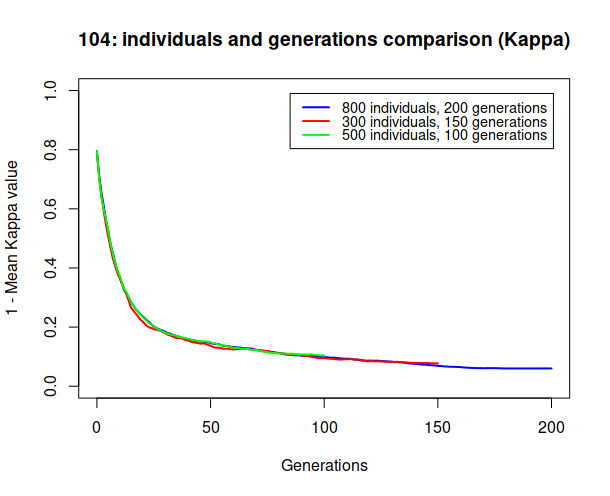
\includegraphics[width=0.45\textwidth]{gfx/FS_IndGens_Kappa_104.png}
				\end{varwidth}
			}
			\fbox{
				\begin{varwidth}{\textwidth}
					\centering
					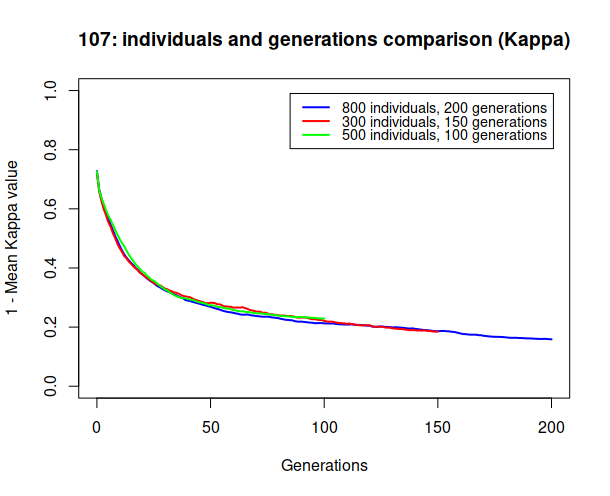
\includegraphics[width=0.45\textwidth]{gfx/FS_IndGens_Kappa_107.png}
				\end{varwidth}
			}
            \fbox{
				\begin{varwidth}{\textwidth}
					\centering
					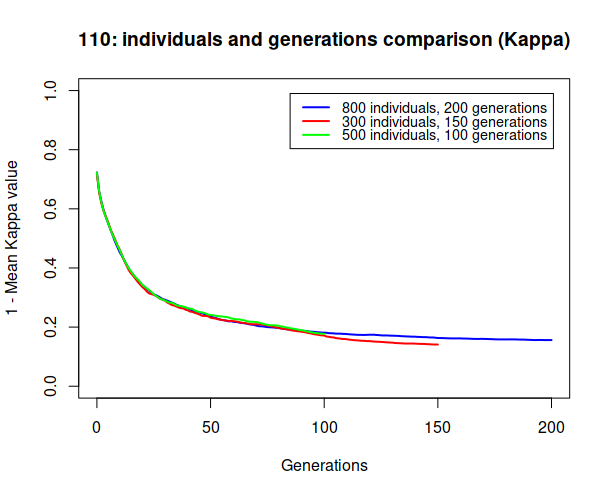
\includegraphics[width=0.45\textwidth]{gfx/FS_IndGens_Kappa_110.png}
				\end{varwidth}
			}

		\end{center}
		\caption[Kappa loss comparison for different populations and generations]{Comparison of Kappa loss evolution over time with different configurations of population and generations.}\label{gfx:fs_popgen_kappa}

	\end{figure}

	There is one definite conclusion we can draw: the number of generations is preventing the emergence of better individuals. The curves follow similar paths until they are progressively stopped by the generation limit. If we take a look at Figure \ref{gfx:fs_popgen_cv}, the same phenomenon is taking place for cross-validation loss, which does not surprise us.

\newpage

	\begin{figure}[bth]

        \begin{center}

        	\setlength{\fboxrule}{0pt}
            \fbox{
				\begin{varwidth}{\textwidth}
					\centering
					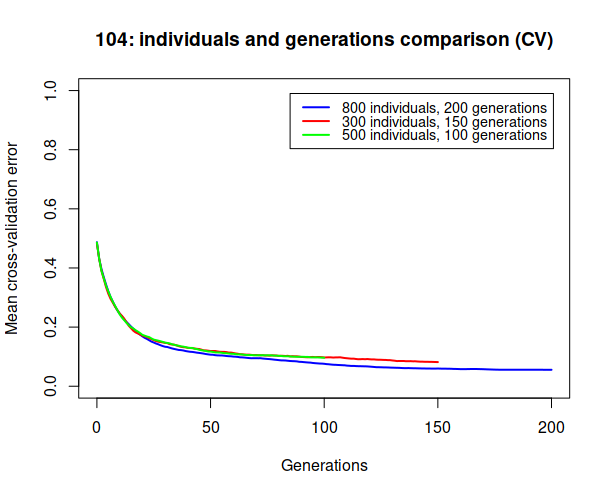
\includegraphics[width=0.45\textwidth]{gfx/FS_IndGens_CV_104.png}
				\end{varwidth}
			}
			\fbox{
				\begin{varwidth}{\textwidth}
					\centering
					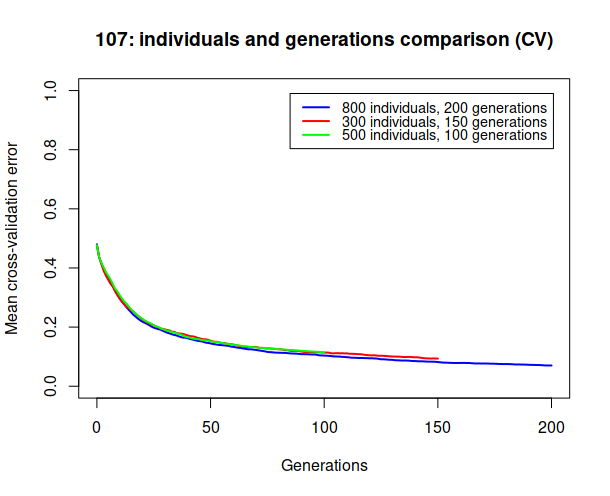
\includegraphics[width=0.45\textwidth]{gfx/FS_IndGens_CV_107.png}
				\end{varwidth}
			}
            \fbox{
				\begin{varwidth}{\textwidth}
					\centering
					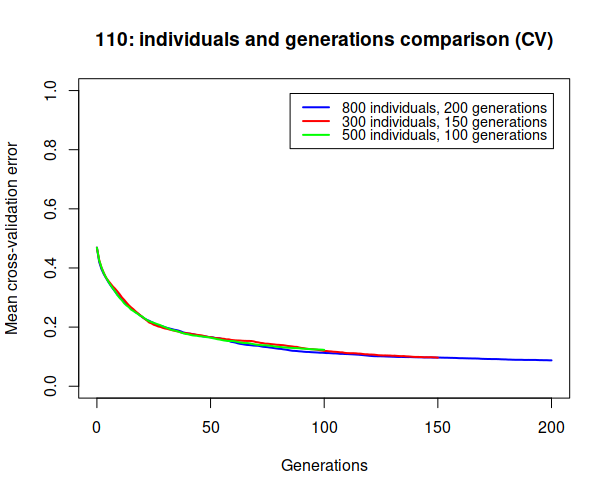
\includegraphics[width=0.45\textwidth]{gfx/FS_IndGens_CV_110.png}
				\end{varwidth}
			}

		\end{center}
		\caption[Cross-validation loss comparison for different populations and generations]{Comparison of cross-validation loss evolution over time with different configurations of population and generations.}\label{gfx:fs_popgen_cv}

	\end{figure}

	It is clear that we need a relevant analysis like that of crossover operators. We will keep the number of individuals intact to grant more diversity, but we have to confirm the importance of extending the evolutionary process. For all this, another 15 algorithm runs for each alternative will be used to make statistical claims.

	First, let us put the average performances alongside one another in Table \ref{table:popgen_kappa}:

	\vspace{0.3cm}

	\begin{table}[h]

        \centering
        \setlength\arrayrulewidth{0.8pt}

        \begin{tabular}{| >{\centering\arraybackslash}m{0.5in} | >{\centering\arraybackslash}m{1.1in} | >{\centering\arraybackslash}m{1.1in} | >{\centering\arraybackslash}m{1.1in} |}

            \hline
            \rowcolor{RoyalBlue}
            \textbf{Subject} & \textbf{300-150} & \textbf{500-100} & \textbf{800-200} \\
            \hline
            \textbf{104} & $0.06534 \pm 0.0074$ & $0.06310 \pm 0.0077$ & $0.05127 \pm 0.0067$ \\
            \hline
            \textbf{107} & $0.15202 \pm 0.0132$ & $0.16830 \pm 0.0145$ & $0.12122 \pm 0.0126$ \\
            \hline
            \textbf{110} & $0.14829 \pm 0.0138$ & $0.15448 \pm 0.0069$ & $0.13369 \pm 0.0083$ \\
            \hline

        \end{tabular}

        \caption{Comparison of average Kappa error values for the three subjects and the three configurations.}\label{table:popgen_kappa}

    \end{table}

    We see that taking the population size up to 800 and the generations up to 200 yields finer average results. It is also noticeable that a bigger population appears to matter less when the number of generations is not accordingly increased.

\newpage

    Tables \ref{table:popgen_kruskal_104}, \ref{table:popgen_kruskal_107} and \ref{table:popgen_kruskal_110} show the Kruskal-Wallis p-values for every pair of combinations. Again, we work with a $95\%$ confidence interval, which means that values below $0.05$ point to statistically significant differences.

    \vspace{0.3cm}

    \begin{table}[h]

        \centering
        \setlength\arrayrulewidth{0.8pt}

        \begin{tabular}{| >{\centering\arraybackslash}m{0.9in} | >{\centering\arraybackslash}m{0.9in} | >{\centering\arraybackslash}m{0.9in} |}

            \hline
            \rowcolor{RoyalBlue}
            \textbf{104} & \textbf{300-150} & \textbf{500-100} \\
            \hline
            \cellcolor{RoyalBlue}\textbf{800-200} & $p = 0.000144$ & $p = 0.000301$ \\
            \hline
            \cellcolor{RoyalBlue}\textbf{300-150} & \cellcolor{lightgray} & \textcolor{red}{$p = 0.884484$} \\
            \hline

        \end{tabular}

        \caption{Comparison of p-values for the evolutionary configurations (subject 104).}\label{table:popgen_kruskal_104}

    \end{table}

    \begin{table}[h]

        \centering
        \setlength\arrayrulewidth{0.8pt}

        \begin{tabular}{| >{\centering\arraybackslash}m{0.9in} | >{\centering\arraybackslash}m{0.9in} | >{\centering\arraybackslash}m{0.9in} |}

        	\hline
            \rowcolor{RoyalBlue}
            \textbf{107} & \textbf{300-150} & \textbf{500-100} \\
            \hline
            \cellcolor{RoyalBlue}\textbf{800-200} & $p = 0.000016$ & $p = 0.000005$ \\
            \hline
            \cellcolor{RoyalBlue}\textbf{300-150} & \cellcolor{lightgray} & $p = 0.002441$ \\
            \hline

        \end{tabular}

        \caption{Comparison of p-values for the evolutionary configurations (subject 107).}\label{table:popgen_kruskal_107}

    \end{table}

    \begin{table}[h]

        \centering
        \setlength\arrayrulewidth{0.8pt}

        \begin{tabular}{| >{\centering\arraybackslash}m{0.9in} |  >{\centering\arraybackslash}m{0.9in} | >{\centering\arraybackslash}m{0.9in} |}

            \hline
            \rowcolor{RoyalBlue}
            \textbf{110} & \textbf{300-150} & \textbf{500-100} \\
            \hline
            \cellcolor{RoyalBlue}\textbf{800-200} & $p = 0.003392$ & $p = 0.000005$ \\
            \hline
            \cellcolor{RoyalBlue}\textbf{300-150} & \cellcolor{lightgray} & $p = 0.034037$ \\
            \hline

        \end{tabular}

        \caption{Comparison of p-values for the evolutionary configurations (subject 110).}\label{table:popgen_kruskal_110}

    \end{table}

    The first thing we notice is that the combination 800-200 is consistently different from the other two. The differences between 300-150 and 500-100 are not so clear at times (see individual 104), but we could say that in a general case the approach with more generations can arrive at better solutions.

    We find ourselves in a quandary between prioritizing computation times or results. The running times are certainly higher with 800-200, but they are still under 2 or 3 hours, which means we can do a lot in a single day. On the side of quality, an improvement of just a few percentage points at this level can be invaluable. Given all this, we will keep the 800-200 configuration and make it our baseline for our forthcoming comparisons against neural networks.

    To wrap up this section, we can foresee that a substantial number of features will lag the already slow training in neural networks. One way to solve this could involve adding a third fitness function to favor individuals with less features. Let us proceed to briefly evaluate this possibility.

    We will use a simple simplicity measure that returns the number of active features of an individual. The goal of the algorithm will be, like with the other two, to minimize it. Sample experiments with and without this simplicity measure can be observed in Figure \ref{gfx:fs_simplicity_kappa}.

    \vspace{0.3cm}

    \begin{figure}[bth]

        \begin{center}

        	\setlength{\fboxrule}{0pt}
            \fbox{
				\begin{varwidth}{\textwidth}
					\centering
					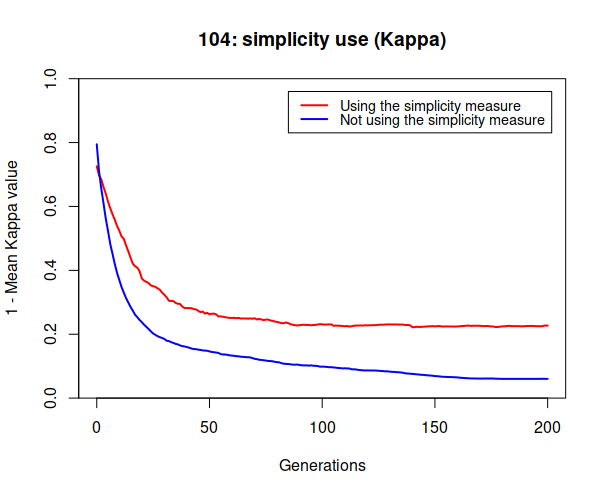
\includegraphics[width=0.45\textwidth]{gfx/FS_Simplicity_Kappa_104.png}
				\end{varwidth}
			}
			\fbox{
				\begin{varwidth}{\textwidth}
					\centering
					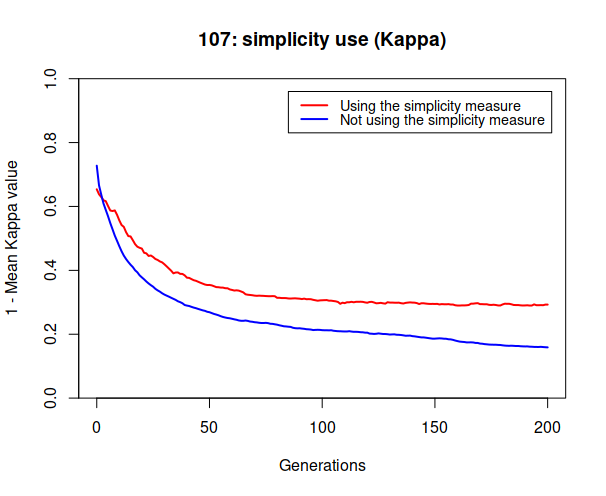
\includegraphics[width=0.45\textwidth]{gfx/FS_Simplicity_Kappa_107.png}
				\end{varwidth}
			}
            \fbox{
				\begin{varwidth}{\textwidth}
					\centering
					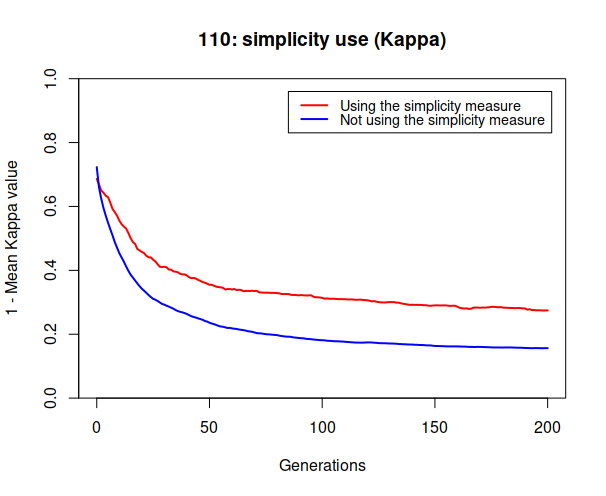
\includegraphics[width=0.45\textwidth]{gfx/FS_Simplicity_Kappa_110.png}
				\end{varwidth}
			}

		\end{center}
		\caption[Kappa loss comparison with and without simplicity]{Comparison of Kappa loss evolution over time with and without the simplicity measure. A similar phenomenon occurs with the cross-validation loss.}\label{gfx:fs_simplicity_kappa}

	\end{figure}

	The reported difference in performance is enormous. There is no need to do any statistical tests to realize that it will keep happening. The explanation is as easy as it gets: the simplicity measure hinders the progress of the other two criteria to the point of ultimately stalling it. In fact, for all we know there might be individuals with just one feature and abysmal accuracy in the first Pareto front.

	In order not to twist the original logic of the algorithm, we will just use the feature cap as a means to keep the number of features under control---more research could be done about where the optimal cap lies.

%\section{Structure optimization}\label{sec:res_so}

%\section{Learning optimization}\label{sec:res_lo}
	\chapter{Conclusions and future work}\label{ch:conclusions}
%************************************************  

\section{Conclusions}

	\subsection{Software developed}

		At the end of this work we have a fully functional codebase \cite{githubrepo} that is theoretically able to address any machine learning problem of the same nature as the one we have attempted to solve here; this means that we can perform a solid feature selection making use of well-established genetic operators and then pass the resulting features on to a two-step neural network optimization method of similar structure if the problem demands so.

		The software is also able to leverage the implicit parallelism in GPUs via \texttt{TensorFlow} and the explicit process distribution to multiple CPU cores and threads, which---only lacking minor technical tweaks---makes for a scalable workflow that can be reused for larger datasets.

		Additionally, the code is written in a modern language like \texttt{Python} and uses popular and up-to-date machine learning and deep learning libraries, which facilitates code maintenance, extensibility and longevity due to the wide community support.

		We can safely state that we have accomplished the purpose of this work, since through the different optimization steps we have been able to choose in a non-arbitrary manner several hyperparameters found in neural networks: the structure (number of inputs and composition of the hidden layers) and three learning parameters (namely, the learning and dropout rates and the number of training epochs). Moreover, the process of designing and writing the necessary code has led to a superior understanding of how the involved technologies work, which was the remaining goal.

	\subsection{The problem tackled in this work}

		The dataset pertains to the area of \acs{BCI}, and in particular it is aimed at telling apart the imagined movements of the left hand, the right hand and the feet. Decisive advances in this classification task have the potential to be useful in medical applications.

		If we assume the accuracy obtained in this work as correct, these results unfold optimistic prospects in terms of practical applications. Although more detailed research is still needed, we can at least say this much. What is more, we have witnessed how \acs{SVM}s---which are not very intricate both in concept and in training---are capable of fulfilling the classification task to an outstanding level.

		Using neural networks in this dataset is perhaps not the most efficient option. Nonetheless, it has allowed us to try the neural network optimization method and conclude that it is powerful enough to be useful.

\section{Future work}

	During the progress of this project many opportunities for further work have appeared. For clarity, we list the most important ones below:

	\begin{itemize}

		\item
		Find the right feature limit in feature selection. Currently, the algorithm tends to use almost as many features as it is allowed; this raises the question of where to put the cap in order to maximize accuracy without losing generalization to unseen data (including the test set).

		\item
		Perform detailed testing of the use of cross-validation against the use of simplicity in the structure optimization phase.

		\item
		Tune the SVM hyperparameter $C$ in order to improve even more its current top accuracy. For this matter we could develop a modified version of the neural network learning optimization or we could use other techniques such as grid search or random search.

		\item
		Try more ambitious learning optimization setups (that is, more individuals and more generations) in order to find out if it yields better models.

		\item
		Find out if there is the possibity of feature transfer between different subjects. This would allow us to skip a big part of the process and make a possible real-world application easier to carry out.

	\end{itemize}

	Less relevant open issues include a better control over randomness in the code or making CPU parallelism a little more robust to increases in the scale of the experiments.



	% Backmatter

	%\appendix
	%\renewcommand{\thechapter}{\alph{chapter}}
	%\cleardoublepage
	%\part{Appendix}
	%\include{Chapters/Chapter0A}
	%********************************************************************
	% Other Stuff in the Back
	%*******************************************************
	\cleardoublepage\defbibheading{bibintoc}[\bibname]{%
  \phantomsection
  \manualmark
  \markboth{\spacedlowsmallcaps{#1}}{\spacedlowsmallcaps{#1}}%
  \addtocontents{toc}{\protect\vspace{\beforebibskip}}%
  \addcontentsline{toc}{chapter}{\tocEntry{#1}}%
  \chapter*{#1}%
}
\printbibliography[heading=bibintoc] 

	\cleardoublepage%*******************************************************
% Declaration
%*******************************************************
\refstepcounter{dummy}
\pdfbookmark[0]{Declaration}{declaration}
\chapter*{Declaration}
\thispagestyle{empty}
\textbf{JAVIER LEÓN PALOMARES} con DNI $00000000$X, actuando en su propio nombre y derecho, \\

\textbf{DECLARA, BAJO SU RESPONSABILIDAD:} \\

Que el Trabajo Fin de Grado presentado en la Escuela Técnica Superior de Ingenierías Informática y de Telecomunicación de la Universidad de Granada, con fecha 18 de junio de 2018, titulado <<\textit{Hyperparameter optimization in Deep Neural Networks, In the context of EEG classification}>> es original, no es copia ni adaptación de ningún otro trabajo, inédito, y no ha sido difundido por ningún medio, ni presentado anteriormente por quien suscribe o por otra persona. \\

Y para que así conste a los efectos oportunos, firmo la presente en Granada, a 18 de junio de 2018.

\bigskip

%\noindent\textit{\myLocation, \myTime}

\smallskip

\begin{flushright}
    \begin{tabular}{m{5cm}}
        \\ \hline
        \centering\myName \\
    \end{tabular}
\end{flushright} 

Asimismo, yo, Javier León Palomares, alumno del Grado en Ingeniería informática de la Escuela Técnica Superior de Ingenierías Informática y de Telecomunicación de la Universidad de Granada, con DNI $00000000$X, autorizo la ubicación de la siguiente copia de mi Trabajo Fin de Grado en la biblioteca del centro para que pueda ser consultada por las personas que lo deseen.

\begin{flushright}
    \begin{tabular}{m{5cm}}
        \\ \hline
        \centering\myName \\
    \end{tabular}
\end{flushright} 
	\cleardoublepage\pagestyle{empty}

\hfill

\vfill


\pdfbookmark[0]{Colophon}{colophon}
\section*{Colophon}
This document was typeset using the typographical look-and-feel \texttt{classicthesis} developed by Andr\'e Miede and Ivo Pletikosić.
The style was inspired by Robert Bringhurst's seminal book on typography ``\emph{The Elements of Typographic Style}''.
\texttt{classicthesis} is available for both \LaTeX\ and \mLyX:
\begin{center}
\url{https://bitbucket.org/amiede/classicthesis/}
\end{center}
Happy users of \texttt{classicthesis} usually send a real postcard to the author, a collection of postcards received so far is featured here:
\begin{center}
\url{http://postcards.miede.de/}
\end{center}
Thank you very much for your feedback and contribution.

\bigskip

\noindent\finalVersionString 


\end{document}
